\documentclass[logo,msc]{infthesis}

% Required by the School template. Do not remove without approval.
\usepackage{msccheck}
% Functional packages only: none overrides margins, font size, or line spacing.
% microtype omitted: it changes \showhyphens and triggers msccheck.
\usepackage{amsmath,amssymb}
\usepackage{booktabs,tabularx,array}
\usepackage{graphicx}
\usepackage{rotating}
\usepackage{url}

\newcolumntype{Y}{>{\raggedright\arraybackslash}X}

\begin{document}
\begin{preliminary}
\title{How Reliable Are LLMs as Cognitive Models? A Systematic Evaluation of Prompt Sensitivity Across Decision-Making Tasks}
% Confirm the author spelling against the University record before submission.
\author{Yijun Chen}
\date{\today}
\abstract{
Large language models (LLMs) are increasingly used to generate measurable experimental behaviour, yet the stability of behavioural conclusions drawn from a single prompt formulation has seldom been examined systematically across models, tasks, and languages. This study operationalises behavioural reliability as the robustness of task-specific conclusions to predefined prompt formulations when task rules and available information are held constant; behavioural similarity is not taken to imply shared human cognitive mechanisms. A Neutral baseline, Instruction specificity, Role framing, and Task-specific construct emphasis were compared in the Horizon Task, Iowa Gambling Task, and Balloon Analogue Risk Task. The English experiment included GPT-4.1, GPT-5.4, and GPT-5.4 Mini; the multilingual experiment fixed GPT-4.1 and analysed English, Simplified Chinese, and Spanish jointly as equally weighted conditions. Each model--language--task--prompt cell contained 20 complete runs, yielding 1,200 unique valid task runs. Analyses estimated raw prompt effects, model-by-prompt interactions, and centred three-language baseline and prompt-effect deviations across eight task-specific metrics. Uncertainty was represented by 2,000 task-appropriate bootstrap replicates, while human-reference proximity was assessed descriptively using human-SD-scaled mean deviations and empirical-interval coverage. Prompt formulations were associated with changes in several behaviours, but effect direction and magnitude varied by model, task, metric, and language implementation; no consistent formulation ranking emerged. Human-reference proximity also changed in some cells, and mean deviation did not invariably track interval coverage. The answer to the title question is therefore conditional: the tested LLMs cannot be treated as reliably prompt-invariant cognitive models, although they can support reproducible measurement of cognitive-task behaviour when the complete measurement specification is fixed, reported, and evaluated for robustness. The principal contribution is an auditable, reviewable multi-task evaluation framework, not evidence of mechanistic or distributional equivalence between LLM runs and human participants.
\par\medskip\noindent\textbf{Keywords:} large language models; prompt sensitivity; behavioural reliability; decision-making tasks; cross-language evaluation; human-reference comparison
}
\maketitle
\standarddeclaration
\tableofcontents
\end{preliminary}

\chapter{Introduction}

Large language models (LLMs) are not only language technologies; they are also increasingly being studied as objects of behavioural experimentation. Researchers have used persona-conditioned LLM responses to simulate respondents with different characteristics \cite{Argyle2023OutOfOneMany}, attempted to reproduce experimental effects previously observed in human participants \cite{Aher2023SimulateHumans}, and treated models as simulated economic agents whose decisions can be examined experimentally \cite{Horton2023HomoSilicus}. Cognitive tasks have likewise been used to characterise behavioural regularities and reasoning biases across GPT models \cite{Binz2023CognitivePsychologyGPT3,Hagendorff2023HumanLikeBiases}. LLMs therefore offer a potentially useful methodological resource: their behaviour can be tested repeatedly under controlled task manipulations.

Nevertheless, a single LLM run is not equivalent to a human participant, and behavioural similarity does not establish a shared cognitive mechanism \cite{Shanahan2023RolePlay}. An LLM output is a conditional sample generated in response to a particular input under specified generation settings. The scientific value of studying an LLM as a cognitive model therefore depends not only on the task-specific behaviour observed, or on its proximity to a human reference sample, but also on whether the resulting conclusions are robust to predefined variations in prompt formulation \cite{Loya2023PromptSensitivityDecision}. In this study, the term \emph{cognitive model} denotes a computational model capable of producing comparable behaviour in cognitive tasks; it does not imply that an LLM possesses the same underlying cognitive mechanisms as humans.

Prompt formulation is central to this question of reliability. A prompt does more than communicate task rules: it can assign the model a role, make particular information salient, and constrain the form of its response. Variations in prompt formulation and generation temperature can alter model performance or choice behaviour \cite{Loya2023PromptSensitivityDecision}. Moreover, framing a model as an experimental participant may elicit a particular simulated identity rather than reveal a stable, context-independent disposition \cite{Shanahan2023RolePlay}. Prompts should therefore be treated as part of the measurement procedure in behavioural research. If prompts that preserve the same task information and rules produce different patterns of exploration, learning, or risk-taking, the resulting conclusions may partly reflect the measurement procedure rather than stable features of the model's behaviour in the target task.

Although previous studies have established that prompting can affect model outputs, the reliability of LLM behaviour has not yet been fully characterised. Many evaluations focus on accuracy, aggregate human similarity, or individual empirical effects, while studies involving multiple prompt templates have primarily examined formatting variations in static benchmarks \cite{Sclar2024PromptFormatting}. Loya et al.~\cite{Loya2023PromptSensitivityDecision} extended this line of inquiry to the sequential Horizon Task, but considered only one decision paradigm. Relatively few studies combine full task runs as the unit of replication; predefined prompt variants that preserve task rules and available information; task- and metric-specific comparisons of model-by-prompt variation under a common implementation; and separate assessments of prompt stability, task-specific behavioural outcomes, and human-reference proximity. Without this combination, it is difficult to determine whether an observed behavioural conclusion reflects a stable feature of a model's task behaviour or a consequence of a particular measurement formulation. These dimensions are not interchangeable: a model may be stable but dissimilar to humans, resemble humans only under a particular prompt, or vary across prompts while maintaining similar average rewards.

Language constitutes a further source of contextual variation. Multilingual evaluations indicate that the performance of a single model may vary substantially across languages and tasks \cite{Ahuja2023MEGA}; evidence obtained in English therefore cannot automatically be generalised to other languages. Interpretable cross-language behavioural comparisons require the model and task environment to be held constant, while task-relevant information and the intended prompt manipulation are aligned across languages. Such alignment does not, however, imply complete pragmatic equivalence among expressions in different natural languages.

This study uses three sequential decision-making tasks. The Horizon Task examines information-seeking choices and changes in exploration across decision horizons \cite{Wilson2014}. The Iowa Gambling Task (IGT) examines longer-term adaptation to reward--loss feedback \cite{Bechara1994}. The Balloon Analogue Risk Task (BART) examines sequential risk-taking in which potential rewards accumulate but the temporary earnings associated with a balloon may be lost if it bursts \cite{Lejuez2002}. Together, these tasks cover exploration, feedback-based learning, and risk management. Participant-level human data are available for each task, permitting descriptive comparisons between human participants and LLM run-level summaries on aligned behavioural metrics \cite{Feng2021ExploreExploit,Steingroever2015IGTData,Sebri2023BART}. Human-reference proximity is used solely as a descriptive behavioural benchmark and not as evidence of shared cognitive mechanisms.

Across the Horizon Task, IGT, and BART, the study compares a Neutral baseline with three manipulated prompt conditions matched on task rules. The conditions preserve the available actions, feedback structure, and boundaries of hidden information, but are not assumed to be pragmatically identical. In particular, the Task-specific construct emphasis condition deliberately changes the salience of concepts relevant to the task. The English-language comparison evaluates prompt sensitivity in GPT-4.1, GPT-5.4, and GPT-5.4 Mini. The cross-language comparison holds the model fixed at GPT-4.1 and compares English, Simplified Chinese, and Spanish. The replication structure and controls applied to the task environments are described in the Method section.

This study makes four principal contributions. First, it defines behavioural robustness as the stability of behaviour across predefined, task-rule-matched prompt conditions, and formulation sensitivity as the magnitude of change relative to the Neutral baseline. Second, it tests, separately for each task and metric, whether prompt effects vary across models and then describes any recurring patterns across tasks. Third, it reports prompt sensitivity, task-specific behavioural outcomes, and human-reference proximity as distinct evaluation dimensions. Fourth, in a multilingual design that holds the model fixed, it locates the baseline behaviour and within-language prompt effects of English, Simplified Chinese, and Spanish jointly within a common centred coordinate system. Because construct emphasis constitutes a substantive manipulation of attentional focus, an effect in that condition is not automatically interpreted as unreliability arising from incidental wording.

The study addresses the following research questions:

\noindent\textbf{RQ1 --- Prompt sensitivity.}
To what extent do Instruction specificity, Role framing, and Task-specific construct emphasis alter a model's task-specific behaviour relative to the Neutral baseline?

\noindent\textbf{RQ2 --- Cross-model variation.}
Within each task and behavioural metric, do the prompt effects of GPT-4.1 or GPT-5.4 Mini differ from those of GPT-5.4? Do the directions and magnitudes of these differences exhibit recurring descriptive patterns across tasks and metrics?

\noindent\textbf{RQ3 --- Cross-language variation.}
When the model, task environment, and generation parameters are held constant, and the intended prompt manipulations and task-relevant information are semantically aligned across languages, do English, Simplified Chinese, and Spanish produce different baseline behaviours or within-language prompt effects?

\noindent\textbf{RQ4 --- Prompt-associated changes in human-reference proximity.}
Relative to the Neutral baseline, do alternative prompt formulations change the absolute human-SD-scaled mean deviation from the human reference mean or the proportion of runs falling within the empirical human reference interval?

RQ4 is explicitly descriptive. Here, ``relative to the Neutral baseline'' refers to comparing the position of each prompt condition with that of the Neutral condition against the same human reference distribution; it does not involve combining Neutral runs with human participants. The corresponding analyses report the signed and absolute human-SD-scaled mean deviations and empirical reference-interval coverage. These quantities are not treated as Cohen's \(d\), are not subjected to binary significance decisions, and are not interpreted as evidence of shared cognitive mechanisms.

Across the model snapshots, tasks, and language implementations examined here, prompt formulations were associated with changes in several task-specific behaviours, but the direction and magnitude of these changes varied by model, task, metric, and language condition. No formulation produced an effect of consistent direction and magnitude across all settings. Direct cross-model interaction contrasts and symmetric, jointly centred three-language comparisons further showed that behavioural conclusions obtained from a single model or a prompt in a single language cannot be assumed to generalise to other models or language conditions. The descriptive human-reference analyses also indicated that prompt formulation could change both the position of the model mean relative to the human mean and the coverage of the empirical human interval by run-level values; these two quantities did not invariably move together. Overall, the robustness of LLM behavioural evidence is conditional on the complete measurement specification, rather than an intrinsic model property separable from the prompt, task, language, and outcome metric. In the sense evaluated here, LLMs are therefore conditionally reliable models of cognitive-task behaviour, not reliably prompt-invariant models of human cognition.

The remainder of this dissertation is organised as follows. Background and Related Work synthesises research on LLM behaviour, prompt sensitivity, cross-model and cross-language variation, sequential decision tasks, and human-reference comparisons, and uses this literature to define the research gap. Method describes the study design, tasks and prompt materials, experimental procedure, data-quality controls, human reference data, behavioural metrics, statistical analyses, and reproducibility boundaries. Results first reports the analysis sample and data quality, then addresses the four research questions through within-model prompt effects, cross-model contrasts, joint three-language centred comparisons, and prompt-associated changes in human-reference proximity. Discussion integrates these findings by considering prompt formulation as part of the behavioural measurement procedure, the methodological contribution of the study, the interpretive limits of human-reference comparisons, and the implications of the study's limitations for replication. Finally, Conclusion and Future Work answers the central research objective, summarises the principal findings and contributions, and identifies priorities for subsequent work.
\chapter{Background and Related Work}

\section{LLMs as Behavioural Experimental Subjects and Computational Models}

Research on LLMs in the behavioural sciences has followed two broad approaches: using models as research tools to simulate participants, and treating models themselves as experimental subjects whose choices and context-dependent responses can be examined using psychological tasks \cite{Dillion2023ReplaceParticipants,Hagendorff2023MachinePsychology,Rahwan2019MachineBehaviour}. The former approach requires the model to support valid inferences about human populations, whereas the latter focuses on the measurable behaviour of a specified computational system. The validation criteria appropriate to these two approaches should not be conflated.

The present study adopts the second approach and defines an LLM as a computational model capable of producing comparable behaviour in cognitive tasks. This is an operational, rather than mechanistic, definition: it does not imply that the model shares human perceptual, learning, or decision-making processes. Research on machine psychology and machine behaviour similarly uses experimental paradigms to characterise artificial systems, but human-like content effects or aggregate behavioural fit may nevertheless arise from different underlying mechanisms \cite{Rahwan2019MachineBehaviour,Lampinen2024ContentEffects,Lin2025SixFallacies}.

This definition also limits the interpretation of LLMs as synthetic participants. Agent architectures incorporating memory, reflection, and planning can produce coherent patterns of behaviour, but those patterns depend on the design of the wider system \cite{Park2023GenerativeAgents}. Synthetic responses may also compress population heterogeneity or lose their original correspondence with human data when the model or prompt is changed \cite{Dillion2023ReplaceParticipants,Bisbee2024SyntheticSurveyData}. Accordingly, the present study examines the behavioural system jointly produced by the model, task, and measurement procedure; it does not treat LLM runs as substitutes for a human population.

\section{Reliability in the Behavioural Measurement of LLMs}

Conventional LLM evaluations often emphasise task accuracy, whereas behavioural experiments must also consider choice distributions, behavioural trajectories, and the extent to which an observed experimental effect depends on a particular measurement formulation. Evaluations using multiple templates indicate that reliance on a single prompt may overstate the certainty of a conclusion, while scoring procedures can themselves introduce apparent variation \cite{Sclar2024PromptFormatting,Mizrahi2024MultiPrompt,Hua2025FlawArtifact}. In this study, \emph{behavioural-measurement reliability} is operationalised as the degree to which the direction and magnitude of a behavioural conclusion remain stable across predefined prompt formulations when the model snapshot, task implementation, generation temperature, response format, and parser are held fixed. This definition does not encompass long-term test--retest reliability across service versions, external validity across other tasks, or the reliability of claims about underlying mechanisms.

The measurement procedure for an LLM includes the prompt, task interface, visible history, output constraints, parser, generation temperature, and deployment state. These components may alter the option produced by the model or affect how its response is parsed and scored \cite{Webson2022PromptMeaning,Sclar2024PromptFormatting,Loya2023PromptSensitivityDecision,Chen2024ChatGPTBehavior,Hua2025FlawArtifact}. A fixed action space and parser can reduce scoring ambiguity, but cannot eliminate the influence of prompt length, informational salience, or information position. Reliable interpretation therefore requires a clear distinction between the elements held constant, those deliberately manipulated, and the scope of the resulting inference.

The unit of analysis is equally important. Repeated runs share model parameters and deployment conditions; variation among them arises from their contexts, task environments, and generation stochasticity. Treating such runs as independent synthetic persons would overstate their population representativeness \cite{Dillion2023ReplaceParticipants,Bisbee2024SyntheticSurveyData}. The present study aligns complete LLM runs with participant-level summaries. It neither treats trials within a run as independent participants nor attributes genuine individual identities to repeated runs.

The coexistence of human--model similarities and differences documented by Lampinen et al.~\cite{Lampinen2024ContentEffects}, together with Lin's distinction between output similarity and mechanistic equivalence \cite{Lin2025SixFallacies}, demonstrates why a single judgement of being ``human-like'' is insufficient for evaluating LLM behavioural evidence. The present study consequently distinguishes three non-interchangeable analytical dimensions: prompt stability, task-specific behavioural outcomes, and human-reference proximity. Stability does not imply that a behaviour is preferable or more human-like, and proximity between means does not establish similarity in distributions or mechanisms. Conclusions should therefore be based on prespecified effect magnitudes, uncertainty, and patterns across metrics, rather than on a single aggregate score or an isolated comparison.

\section{Prompt Sensitivity and Behavioural Variation}

Research on prompt sensitivity has shown that label bias, demonstration order, formatting, and option order can all alter model outputs \cite{Zhao2021Calibrate,Lu2022PromptOrder,Sclar2024PromptFormatting,Pezeshkpour2024OptionOrder}. The observation that irrelevant or misleading instructions can still produce high task scores further indicates that successful performance does not necessarily demonstrate a stable understanding of the task \cite{Webson2022PromptMeaning}. The prompt must therefore be regarded as part of the behavioural measurement procedure.

The field has accordingly begun to move from searching for a single ``best prompt'' towards multi-prompt evaluation and instance-level quantification of sensitivity \cite{Mizrahi2024MultiPrompt,Zhuo2024ProSA}. Much of this evidence, however, comes from static benchmarks or single-round task responses. Loya et al.~\cite{Loya2023PromptSensitivityDecision} found that choices in the Horizon Task varied with prompts and generation temperature across three OpenAI models, but examined only one sequential decision paradigm and did not include a multilingual comparison.

The interpretation of a prompt effect depends on the type of manipulation involved. Formatting and label-order manipulations primarily test sensitivity to incidental design features, whereas role-play prompting has also been shown to alter model performance across several reasoning benchmarks \cite{Kong2024RolePlayPrompting}. In the present study, Instruction specificity, Role framing, and Task-specific construct emphasis are predefined as substantively meaningful manipulations that may affect rule representation, role context, or conceptual salience. Their behavioural consequences in sequential decision tasks remain empirical questions. Because these formulations also differ in length, keywords, and information position, the complete formulation is the object of inference. These correlated presentational differences constitute a design limitation and cannot be decomposed retrospectively from the observed condition effect. Consequently, a condition effect should not automatically be characterised as unreliability caused by irrelevant wording \cite{Sclar2024PromptFormatting,Hua2025FlawArtifact}.

\section{Model Variation and Reproducibility in LLM Behavioural Measurement}

Behavioural measurements are not necessarily invariant across models. Multi-model evaluations indicate that both baseline performance and prompt sensitivity may differ among models \cite{Sclar2024PromptFormatting,Mizrahi2024MultiPrompt,Zhuo2024ProSA}. A comparison of model means in a single condition cannot distinguish an overall behavioural difference from differential formulation sensitivity. It is therefore necessary first to estimate the condition-minus-baseline effect for each model and then to compare those effects directly.

Cross-model comparisons are also affected by changes in model services. Proprietary services and model versions may change over time, often through opaque update processes, and the same model name does not guarantee identical behaviour at different collection dates \cite{Chen2024ChatGPTBehavior}. Palmer, Smith and Spirling~\cite{Palmer2024ProprietaryModels} accordingly emphasise the transparency and reproducibility constraints associated with proprietary language models. The present study records requested and resolved model identifiers, collection dates, generation settings, prompt versions, and failure logs. Using fixed model snapshots can reduce, but cannot eliminate, temporal drift.

Taken together, this evidence indicates that cross-model behavioural comparisons should examine both baseline behaviour and formulation sensitivity, while restricting inference to the model versions actually tested \cite{Chen2024ChatGPTBehavior,Palmer2024ProprietaryModels}. Differences should not be interpreted as causal effects of architecture or scale. The models, reference directions, and generation settings used in the present study are specified in the Method section.

\section{Language Effects in LLM Behavioural Measurement}

The multilingual capabilities of an LLM are not proportional replications of its capabilities in English. Cross-language benchmarks show that accuracy and performance on culturally situated knowledge vary across languages and task levels. Moreover, improvements in a larger model's average multilingual performance do not necessarily produce greater cross-lingual consistency \cite{Zhang2023M3Exam,Qi2023CrossLingualConsistency}. Support for a language therefore does not imply that the same behavioural experiment has identical measurement properties in that language, and findings obtained in English cannot automatically be generalised to Chinese or Spanish.

Existing multilingual research has primarily used translated benchmarks, cross-lingual prompting, or multilingual chain-of-thought methods. Instruction tuning in English can transfer to other languages, but the degree of transfer depends on factors including pre-training coverage, task format, the language of demonstrations, and the reasoning strategy employed \cite{Muennighoff2023CrosslingualGeneralization,Shi2023MultilingualCoT}. Performance may also vary according to how instructions, contexts, examples, and output components are translated \cite{Mondshine2025BeyondEnglish}. These approaches have less often examined both the baseline behaviour and within-language prompt effects of a fixed model completing full behavioural task runs.

Such cross-language differences also make prompt translation an experimental operation in its own right. Semantic alignment does not guarantee identical measurement properties, because translation quality, linguistic distance from English, and pre-training coverage may all affect model behaviour \cite{Mondshine2025BeyondEnglish}. The present study therefore requires task-relevant informational equivalence rather than complete semantic or pragmatic equivalence across language versions. Observed differences are interpreted cautiously as language-associated differences specific to the tested model, translation, and task implementation. The translation review procedure and statistical contrasts are specified in the Method section.

\section{Sequential Decision Tasks and Their Cognitive Constructs}

In each of the three tasks selected for this study, a current choice and the feedback subsequently presented contribute jointly to a behavioural trajectory across trials or steps. This structure makes it possible to examine how the model uses previous information and adjusts later choices \cite{Wilson2014,Bechara1994,Lejuez2002,Loya2023PromptSensitivityDecision}. Because of this trajectory dependence, the complete run is used as the analysis unit; trials within the same run are not treated as independent participants.

The Horizon Task uses information asymmetry and the number of remaining decision opportunities to examine the explore--exploit dilemma \cite{Wilson2014}. Directed and random exploration can produce superficially similar choices while corresponding to different computational descriptions \cite{Gershman2018Exploration}. The information-seeking choice rate, horizon-related exploration change, and model-derived decision-noise difference should therefore be interpreted separately.

The IGT was originally developed to examine how repeated reward and loss feedback shapes subsequent choice \cite{Bechara1994}. However, the same eventual deck preference may arise from different patterns of outcome valuation, learning, and response consistency \cite{Busemeyer2002PVL,Steingroever2013PVLDelta}. Reviews of its construct validity likewise caution against treating an aggregate IGT score as a unitary measure of decision-making ability \cite{Buelow2009IGTValidity}. For an LLM, the explicit presentation of cumulative or average outcomes may impose a lower memory demand than the classic human task. Interpretation must therefore remain limited to the behavioural metrics aligned across implementations.

The BART examines sequential risk-taking and stopping behaviour by increasing potential gains while simultaneously increasing the risk of an explosion \cite{Lejuez2002}. The number of pumps is not a pure measure of risk preference; it may also reflect learning about explosion probabilities and response consistency \cite{Wallsten2005BARTModel,VanRavenzwaaij2011BART}. The present study therefore reports adjusted pumps, explosion rate, and post-explosion adjustment as complementary indicators. Although the three tasks address exploration, feedback-based learning, and risk-taking, respectively, they differ in their constructs, measurement scales, and feedback structures. Each task and metric is consequently analysed separately, and no aggregate score of general ``decision-making ability'' is constructed.

\section{Human-Reference Comparisons: Purpose and Limits}

Human-reference comparisons can describe where a model lies relative to an empirical human reference on a particular metric. The present analysis distinguishes the position of the model mean, the proportion of runs falling within the empirical human reference interval, and the response to an experimental manipulation. These quantities answer different questions and are not substitutes for one another. Humans and models may exhibit a similar aggregate effect while differing in task-specific behaviour \cite{Lampinen2024ContentEffects}, and correspondence at the output level does not demonstrate mechanistic equivalence \cite{Lin2025SixFallacies}. Human-reference proximity is therefore treated as a descriptive behavioural reference, not as a test of cognitive equivalence or shared mechanisms.

These comparisons are also constrained by the units of analysis and the degree of task alignment. An LLM run can be operationally aligned with a participant-level summary, but it is not an independent human individual; repeated runs share model parameters and deployment conditions \cite{Dillion2023ReplaceParticipants,Bisbee2024SyntheticSurveyData}. Differences in task length, information presentation, and familiarisation are treated as design-alignment limitations, and comparisons are restricted to metrics that can be aligned across the LLM and human implementations \cite{Wilson2014,Buelow2009IGTValidity,Wallsten2005BARTModel}. A mean deviation and empirical reference-interval coverage describe, respectively, relative mean position and the proportion of LLM runs within a prespecified human interval; they need not support the same descriptive conclusion.

The human reference is not a normative performance target. The direction of the IGT advantageous-choice rate is comparatively interpretable, but neither the number of BART pumps nor information seeking has a single context-independent optimum. Greater proximity to the human mean therefore does not automatically indicate improved decision quality \cite{Wilson2014,Buelow2009IGTValidity,Wallsten2005BARTModel}. The signed human-SD-scaled mean deviation, its absolute value, and empirical interval coverage are consequently reported as complementary supplementary or descriptive measures. They are not treated as Cohen's \(d\), evidence of overall equivalence, or evidence of a shared mechanism.

\section{Research Gap and Positioning of the Present Study}

Existing research has established several relevant lines of inquiry, including synthetic-participant simulation, machine psychology, prompt-robustness evaluation, and multilingual benchmarking. These approaches have generally pursued different objectives, such as population simulation, performance on individual benchmark items, the reproduction of particular psychological effects, or aggregate accuracy \cite{Dillion2023ReplaceParticipants,Hagendorff2023MachinePsychology,Mizrahi2024MultiPrompt,Zhang2023M3Exam}. Collectively, they demonstrate that LLM behaviour can be investigated experimentally, but they do not integrate measurement stability, task-specific behaviour, and human-reference proximity within a common evaluation design.

Some existing studies include multiple models or multiple prompt variants, but their evidence is drawn mainly from static benchmarks or from a single sequential decision task. Studies of multilingual consistency, meanwhile, typically use separate factual-knowledge or benchmark settings \cite{Loya2023PromptSensitivityDecision,Sclar2024PromptFormatting,Qi2023CrossLingualConsistency}. Within the literature reviewed here, no study was identified that combines, within a single design, full sequential task runs, controlled prompt variants, multiple models, multiple decision constructs, and a cross-language comparison holding the model fixed. The available evidence is therefore insufficient to establish whether behavioural conclusions remain robust across these prompt formulations, model versions, and language implementations.

The present study combines controlled multi-prompt evaluation with full sequential task runs and extends this approach across tasks, models, and languages \cite{Loya2023PromptSensitivityDecision,Sclar2024PromptFormatting,Mizrahi2024MultiPrompt}. It also distinguishes formulation stability, task-specific behavioural outcomes, and human-reference proximity. Its contribution is not to determine whether LLMs are globally ``like humans'', but to assess systematically whether conclusions about their behaviour in cognitive tasks remain robust across predefined variations in prompts, models, and languages.
\chapter{Method}

\section{Study Design and Scope}

This study used a controlled repeated-run design to examine whether prompt formulation altered LLM behaviour in cognitive decision tasks when task rules, environmental parameters, and available information were held constant. Two complementary comparisons were analysed separately. An English-language, three-model comparison tested whether prompt sensitivity varied by model and task. A three-language comparison held the model fixed at GPT-4.1 and tested whether semantically aligned English, Simplified Chinese, and Spanish prompts produced different baseline behaviour or prompt effects.

GPT-4.1, GPT-5.4, and GPT-5.4 Mini each completed the Horizon Task, Iowa Gambling Task (IGT), and Balloon Analogue Risk Task (BART) under four prompt conditions: Neutral baseline, Instruction specificity, Role framing, and Task-specific construct emphasis. The English comparison comprised $3$ models $\times$ $3$ tasks $\times$ $4$ conditions $\times$ $20$ valid runs, yielding 720 valid task runs. The multilingual comparison used \texttt{gpt-4.1-2025-04-14} in $3$ languages $\times$ $3$ tasks $\times$ $4$ conditions $\times$ $20$ valid runs, also yielding 720 runs. The 240 English GPT-4.1 runs were shared between the two comparisons rather than collected twice; the study therefore contained 1,200 unique valid task runs, not 1,440. Accordingly, the English GPT-4.1 results in the two designs are not independent replications. Figure~\ref{fig:study_design_scope} shows the shared task and condition structure, the two comparison paths, and their connection through the common English GPT-4.1 sample; the complete factorial expansion is provided in the technical appendix.

\begin{figure}[htbp]
\centering

\includegraphics[width=0.98\textwidth]{outputs/figures/design/study_design_scope.png}
\caption{Study design and deduplicated data structure. The shared English GPT-4.1 sample is counted once.}
\label{fig:study_design_scope}
\end{figure}

The target of 20 complete runs per cell was fixed by the available computational budget rather than by a conventional power calculation. Incomplete or unparseable runs did not count towards this target and were replaced under the same technical criteria until each cell contained 20 valid runs. Inclusion did not depend on behavioural direction, extremity, ceiling or floor effects, or zero variance. The analysis therefore emphasised effect direction, magnitude, and precision; a wide interval was not interpreted as evidence of no prompt effect. Failure records, replacement runs, and fitting diagnostics are reported in the technical appendix.

All three languages used the same task implementations, parameters, generation settings, response formats, and matched base seeds. The Chinese and Spanish versions preserved the rules, task-relevant information, intended manipulation, and response requirements of the canonical English versions, although complete pragmatic equivalence was not assumed. A complete task run was the primary statistical unit. Trials, choices, games, and balloons were observations nested within runs and were used to calculate task-specific metrics or, where required, fit choice models. Run-level metrics were then compared by model, task, and prompt condition. For human-reference analyses, a complete LLM run was treated as a participant-level behavioural analogue, not as a human participant.

Prompt sensitivity was defined as behavioural variation associated with a prespecified change in prompt formulation while the rules, environmental parameters, available actions, feedback structure, and boundaries of hidden information remained fixed. Each manipulated condition was compared with the Neutral baseline for the same model and task. The four formulations were not assumed to be pragmatically identical: Instruction specificity expanded the rules, Role framing changed the role context, and Task-specific construct emphasis deliberately increased the salience of task-relevant concepts. Condition effects were therefore interpreted as sensitivity to the formulation as a whole, rather than attributed indiscriminately to theoretically irrelevant surface wording.

Reliability refers here specifically to behavioural robustness: whether task-specific conclusions about model behaviour remain stable across prespecified formulations that preserve the task rules and available information. Large prompt effects, reversals across conditions, or marked changes in position relative to the human reference indicate formulation-dependent conclusions. Prompt stability does not itself imply better task performance or a shared cognitive mechanism. Cross-language versions were aligned in task-relevant content and intended manipulation, but not assumed equivalent in every pragmatic feature or degree of informational salience.

\section{Models and API Configuration}

All models were accessed through the OpenAI-compatible Responses API endpoint provided by the University of Edinburgh ELM platform. GPT-4.1 served as a reference model; GPT-5.4 represented a newer frontier general-purpose model; and GPT-5.4 Mini represented a compact model designed for lower latency, lower cost, and higher throughput. Their inclusion tested model variation in prompt sensitivity, not overall capability rankings. Because model size, full architecture, training-token count, and corpus composition are not publicly disclosed, no unverified third-party estimates were used and observed differences were not attributed simply to parameter count.

All models used identical task implementations, prompt conditions, response constraints, and repeated-run procedures. Generation settings were \texttt{temperature = 0.7}, \texttt{top\_p = 1.0}, and \texttt{max\_output\_tokens = 16}. GPT-5.4 and GPT-5.4 Mini used \texttt{reasoning\_effort = none}; GPT-4.1 used its standard non-reasoning configuration. The ELM API did not expose a controllable token-sampling seed. Task-environment seeds therefore controlled environmental randomisation, but not model-generation randomness.

\begin{table}[htbp]
\centering
\caption{Model identifiers and formal data-collection periods.}
\label{tab:model_identifiers}
\begin{tabularx}{\textwidth}{@{}>{\raggedright\arraybackslash}p{2.1cm}>{\raggedright\arraybackslash}X>{\raggedright\arraybackslash}X>{\raggedright\arraybackslash}p{3.2cm}@{}}
\toprule
\textbf{Model} & \textbf{Requested identifier} & \textbf{Resolved identifier} & \textbf{Collection period} \\
\midrule
GPT-4.1 & \texttt{gpt-4.1-2025-04-14} & \texttt{gpt-4.1-2025-04-14} & English: 8--13 July 2026; zh-CN: 3--5 August 2026; es: 5--7 August 2026 \\
GPT-5.4 & \texttt{gpt-5.4} & \texttt{gpt-5.4-2026-03-05} & 30--31 July 2026 \\
GPT-5.4 Mini & \texttt{gpt-5.4-mini} & \texttt{gpt-5.4-mini-2026-03-17} & 1 August 2026 \\
\bottomrule
\end{tabularx}
\end{table}

Dates are formal output-generation dates in the Asia/Shanghai time zone. GPT-4.1 data were collected in separate language batches; possible provider-side temporal drift is addressed under Reproducibility.

\section{Decision-Making Tasks}

Three established sequential tasks examined exploration--exploitation, feedback-based choice learning, and risk-taking. At each step, the model received the current state and previous feedback and selected from a constrained action set. The environment parsed the response, updated its state, and returned the outcome. Hidden parameters and future outcomes were unavailable beyond the rules and information needed for the current choice.

\subsection{Horizon Task}

The implementation followed the core design of the Horizon Task~\cite{Wilson2014}. Each run contained 40 independent two-option games, with options labelled A and B. Four forced choices preceded the free-choice phase. Horizon~1 contained one free choice (five choices in total), whereas Horizon~6 contained six (ten choices in total). The model saw the game and choice numbers, remaining choices, observed rewards, and the currently required option during forced trials. It could infer horizon from the remaining choices, but did not see the internal labels \texttt{horizon\_1} or \texttt{horizon\_6}.

Each horizon included equal- and unequal-information games. Equal-information games forced two observations of each option. Unequal-information games forced one observation of one option and three of the other; the less-observed option was randomly assigned to A or B, and forced-choice order was randomised. The model saw each option's reward history, but not internal condition labels. The 40 games followed a fixed balanced order across the four horizon-by-information combinations, with ten games per combination: horizons alternated by game and information condition changed every two games. The environment seed controlled assignment of the less-observed option, forced-choice order, hidden reward means, and sampled rewards, but not condition counts or order.

At the start of each game, an anchor mean $\mu_{\mathrm{anchor}}$ was sampled from $\{40,60\}$ and a non-zero difference $\Delta\mu$ from $\{-30,-20,-12,-8,-4,4,8,12,20,30\}$. The two latent means were the anchor and the anchor plus this difference, randomly assigned to A and B; both therefore lay between 10 and 90. Rewards were sampled from the corresponding Gaussian distribution with standard deviation 8, rounded to integers, and clipped to $[1,100]$. Latent means were never disclosed. The same seed reproduced the forced-choice sequence, latent means, and potential reward sequence, although divergent free choices could still produce different observed histories.

\subsection{Iowa Gambling Task}

The IGT examined whether repeated reward and loss feedback produced an increasing preference for advantageous long-run choices~\cite{Bechara1994}. Each run comprised 100 choices and began with 2,000 points. Decks A and B yielded 100 points per selection and decks C and D yielded 50. Deterministic loss schedules repeated every ten selections from a given deck. A and B each produced a net $-250$ per ten selections; C and D each produced $+250$. A and C had relatively frequent losses, whereas B and D had rarer but larger losses.

These long-run properties were undisclosed. After each choice, the model received the deck, reward, signed loss, net outcome, and updated total. Subsequent observations also contained the preceding trial's complete outcome, choice counts and cumulative and mean net outcomes by deck, and results from the five most recent trials. These summaries reduced the need to remember and integrate the entire history and are not normally provided in equivalent form to human IGT participants. The implementation was therefore treated as an LLM-adapted IGT. Human comparisons concerned aligned observable choice metrics only, not identical memory demands or an unqualified learning-capacity difference. The 100 trials were continuous: score, deck counts, and payoff schedules were never reset. The fixed schedule used no environmental randomisation; outcomes depended only on the cumulative number of selections from each deck within its repeating ten-choice cycle.

\subsection{Balloon Analogue Risk Task}

The BART examined risk-taking when potential gain increases with action while failure risk accumulates~\cite{Lejuez2002}. Each run contained 40 balloons, recorded in two consecutive 20-balloon blocks; blocks did not alter balloon generation or available actions. The model chose \texttt{PUMP} or \texttt{CASH\_OUT}. Each successful pump added 0.05 to the balloon's temporary value. Cashing out banked that value; an explosion forfeited it and advanced to the next balloon.

Explosion points were generated from the environment seed at run initialisation. At pump $k$,
\[
P(\text{explosion at pump }k\mid\text{survival through pumps }1,\ldots,k-1)=\frac{1}{33-k},\qquad k=1,\ldots,32.
\]
Risk therefore increased with pump count, with certain explosion at pump 32. The model was told only that pumping could cause an explosion and that balloons could differ. Before each decision it saw balloon and block number, current pump count, temporary value, and cumulative total. After at least one completed balloon, it also saw the preceding balloon's pump count, outcome and payoff; the five most recent balloon outcomes; and cumulative explosions and mean pumps. Forty latent explosion points were generated per run, and identical seeds yielded identical potential sequences.

\section{Prompt Construction and Validation}

\subsection{Prompt Conditions}

The Neutral baseline gave concise, neutral instructions containing only the necessary rules, actions, and response requirements. Instruction specificity stated the same rules and procedures more explicitly without adding task information. Role framing asked the model to act as a human participant, without asking it to mimic typical human behaviour or supplying a strategy. Task-specific construct emphasis highlighted uncertainty and information acquisition in the Horizon Task, reward and loss feedback in the IGT, and risk-taking and risk management in BART. It increased the salience of concepts already present in the baseline without revealing hidden parameters or prescribing choices.

Within each task, rules, actions, feedback, payoff schedule, task length, response format, and hidden-information boundary were held constant. Conditions used independent contexts. Prompt lengths were not artificially matched: specificity necessarily expanded and repeated rules, whereas framing and construct emphasis altered keyword salience and position. Frozen texts and character counts were retained. Because the endpoint provided no verifiable static token breakdown, and its proprietary tokenisers could not be assumed to match public tokenisers, estimated token counts were not treated as exact covariates. Effects consequently pertain to the controlled formulation as a whole and cannot isolate length, repetition, keyword salience, or a single linguistic feature.

\subsection{Prompt Development and Validation}

The researcher constructed the three canonical baselines from the original task literature and implemented task rules. Nine variants were then produced by constrained rewriting under a prespecified controlled-variant protocol, using low-variability generation settings but no controllable sampling seed. Candidates were manually checked against their baselines for rules, actions, feedback, hidden-information boundaries, response requirements, and intended manipulation, and screened for unintended information or strategy advice. Pretesting established compatibility with task flow and response parsing. This supported task-rule alignment but did not establish identity on every non-target linguistic feature. The three baselines and nine variants were frozen before data collection and used unchanged across the three models; full texts, generation settings, review records, and version identifiers are provided in the appendix.

\subsection{Multilingual Prompt Construction and Validation}

English was the canonical source. Twelve Simplified Chinese and twelve Spanish prompts mapped to the same task-condition combinations, preserving rules, actions, feedback, hidden-information boundaries, manipulation intent, and response format while avoiding additional strategy advice, cultural framing, or explanation. Target-language baselines were generated under written translation constraints; variants were derived from the reviewed baseline in the same language. The researcher used a common checklist and AI-assisted semantic review to identify omissions, additions, between-condition information asymmetry, manipulation drift, and changes to numbers, payoff rules, hidden-information boundaries, or response formats; all final decisions were made by the researcher. There was neither independent bilingual validation nor independent back-translation. The procedure therefore supports task-relevant informational equivalence, not complete equivalence in naturalness, cultural appropriateness, length, vocabulary, syntax, or pragmatics. Action labels, response formats, task parameters, and numerical rules were identical; static instructions and dynamic observations were presented in the target language. Materials were frozen before collection.

\section{Experimental Procedure and Data Quality}

Figure~\ref{fig:experimental_workflow} summarises the sequence from frozen materials to formal analysis. Each run used an independent context and repeated observation--response--update cycles; inclusion required a complete record, and technical failures were handled under outcome-independent prespecified rules.

\begin{figure}[htbp]
\centering

\includegraphics[width=0.98\textwidth]{outputs/figures/design/experimental_workflow.png}
\caption{Experimental workflow from frozen materials to formal analysis.}
\label{fig:experimental_workflow}
\end{figure}

\subsection{Run Procedure}

The cross-model experiment targeted 20 complete valid runs per model--task--condition cell. The multilingual experiment fixed GPT-4.1 and used the same $3$ tasks $\times$ $4$ conditions $\times$ $20$ matched base seeds in each language. Runs, conditions, and languages shared no conversational history. At every decision, the current observation was inserted into the frozen template and submitted as a separate API request. The environment parsed the action, updated the state, and generated the next observation. Previous choices and feedback were supplied through deterministic state and history fields, not a persistent conversation or model-generated summary. Because task progress changed observation length and formulations differed in length, total context length was not exactly matched.

Horizon and BART seeds controlled environmental randomisation. A common seed supplied comparable initial environments across models, conditions, and languages, but did not guarantee identical realised feedback after choices diverged. The IGT had a fixed payoff schedule; nominal seeds only identified corresponding runs and did not justify paired-seed inference. Each run retained model responses, parsed actions, and its complete task record. Environmental seeds did not control token sampling, for which the API exposed no seed.

\subsection{Response Parsing and Quality Control}

Strict task-specific parsers required \texttt{CHOICE: A} or \texttt{CHOICE: B} in Horizon; \texttt{CHOICE: A}, \texttt{B}, \texttt{C}, or \texttt{D} in IGT; and \texttt{ACTION: PUMP} or \texttt{ACTION: CASH\_OUT} in BART. Parsing was case-insensitive, ignored surrounding whitespace, and accepted a valid response enclosed by a complete Markdown code fence; it did not infer or repair invalid actions from context. One repeat request was prespecified after an initial parse failure, with prompt, observation, and task state unchanged. Invalid responses did not advance the task. A second failure or unrecoverable service error rendered the run incomplete. Only runs completing the prescribed structure with complete records and the prespecified configuration entered analysis. Successfully retried complete runs were retained; valid extreme, ceiling, floor, and zero-variance behaviour was not excluded.

\section{Human Reference Data}

One existing dataset per task supplied a descriptive human reference distribution. Selection required sufficient task comparability, trial-level records for the primary metrics, and participant-level behavioural summaries. Human data were neither normative targets nor evidence of a shared latent mechanism.

Horizon data came from Feng et al.~\cite{Feng2021ExploreExploit} and comprised 60 participants with complete choice records. Each completed 320 games, compared with 40 per LLM run; metric definitions were aligned, but measurement precision and sampling variation were not. IGT data came from Steingroever et al.~\cite{Steingroever2015IGTData}: the 100-trial subset with complete choice, reward, and loss records comprised 504 healthy participants. BART data came from the public 40-balloon dataset of Sebri et al.~\cite{Sebri2023BART}. Excluding six participants aged under 18 left 141 adults; 140 contributed to post-explosion adjustment because one had no eligible transition. The LLM and human BART versions shared 40 balloons in two 20-balloon blocks, a 0.05 increment per successful pump, and explosion probability $1/(33-k)$ at pump $k$ (certain explosion at 32). The source study included familiarisation, whereas the LLM implementation had no practice balloons and supplied structured recent and cumulative information. Comparisons were therefore restricted to alignable pumping and explosion measures. Human records were converted to participant-level summaries using the LLM definitions, and participants were not pooled across tasks.

\section{Statistical Analysis}

\subsection{Behavioural Metrics}

Seven metrics were calculated directly from each complete run. Random exploration was estimated jointly within each model--language--prompt cell using a first-free-choice hierarchical logistic choice model, producing one cell estimate and partially pooled run estimates.

\begin{table}[htbp]
\centering
\caption{Primary behavioural metrics and participant/run-level operational definitions.}
\label{tab:behavioural_metrics}
\begin{tabularx}{\textwidth}{@{}p{1.7cm}p{3.6cm}X@{}}
\toprule
\textbf{Task} & \textbf{Metric} & \textbf{Operational definition} \\
\midrule
Horizon & Information-seeking choice rate & Proportion of first free choices in unequal-information games selecting the less-observed option. \\
Horizon & Horizon-related exploration change & Horizon~6 minus Horizon~1 first-free-choice exploration rate, including both information conditions and excluding observed-mean ties. \\
Horizon & Random exploration effect & Horizon-specific decision-noise difference estimated by the hierarchical first-free-choice logistic model. \\
IGT & Advantageous choice rate & Proportion of 100 trials selecting C or D. \\
IGT & Post-loss switching rate & Proportion of eligible trials with a signed loss component below zero followed by a switch of deck. \\
BART & Adjusted average pumps & Mean pumps among non-exploded balloons. \\
BART & Explosion rate & Proportion of all balloons that exploded. \\
BART & Post-explosion adjustment & Mean difference between pumps on the balloon after an explosion and pumps on the exploded balloon. \\
\bottomrule
\end{tabularx}
\end{table}

Adjusted pumps conditions on balloon survival, so differences may reflect both pumping policy and which balloons enter the denominator; it was interpreted alongside explosion rate. The metrics jointly cover information seeking, horizon-related value-based exploration, random exploration, advantageous learning, immediate loss response, pumping persistence, realised explosions, and post-explosion adjustment. They are observable run summaries or prespecified model estimates and do not rely on self-reported strategy. Information-seeking rate is not the classic horizon-dependent directed-exploration effect.

For participant/run $i$ and $h\in\{\mathrm{H1},\mathrm{H6}\}$, let $E_{i,h}$ be the proportion of eligible first free choices selecting the option with the lower pre-choice observed mean. Equal- and unequal-information games were included; observed-mean ties were excluded from numerator and denominator. Then
\[
\mathrm{HorizonEffect}_{i}=E_{i,\mathrm{H6}}-E_{i,\mathrm{H1}}.
\]
A positive value denotes more such value-based exploratory choices at the longer horizon. This is neither a horizon difference in information-seeking rate nor an analysis of free choices two to six. If either horizon had no eligible non-tied first free choices, the metric was missing rather than zero.
One existing dataset per task supplied a descriptive human reference distribution. Selection required sufficient task comparability, trial-level records for the primary metrics, and participant-level behavioural summaries. Human data were neither normative targets nor evidence of a shared latent mechanism.

Horizon data came from Feng et al.~\cite{Feng2021ExploreExploit} and comprised 60 participants with complete choice records. Each completed 320 games, compared with 40 per LLM run; metric definitions were aligned, but measurement precision and sampling variation were not. IGT data came from Steingroever et al.~\cite{Steingroever2015IGTData}: the 100-trial subset with complete choice, reward, and loss records comprised 504 healthy participants. BART data came from the public 40-balloon dataset of Sebri et al.~\cite{Sebri2023BART}. Excluding six participants aged under 18 left 141 adults; 140 contributed to post-explosion adjustment because one had no eligible transition. The LLM and human BART versions shared 40 balloons in two 20-balloon blocks, a 0.05 increment per successful pump, and explosion probability $1/(33-k)$ at pump $k$ (certain explosion at 32). The source study included familiarisation, whereas the LLM implementation had no practice balloons and supplied structured recent and cumulative information. Comparisons were therefore restricted to alignable pumping and explosion measures. Human records were converted to participant-level summaries using the LLM definitions, and participants were not pooled across tasks.
In the IGT, \texttt{loss} is signed: zero denotes no loss and negative values denote a loss. Post-loss switching used \texttt{loss < 0}, not net outcome or \texttt{loss > 0}. Thus a trial remained a loss event when its positive reward made its net outcome non-negative. For eligible $t<100$, switching at $t+1$ was averaged; trial 100 was excluded because it had no subsequent choice.

Random exploration used only each game's first free choice. Let $p_{ig}$ be the probability that run $i$ chooses A in game $g$, with horizon $h$:
\[
\operatorname{logit}(p_{ig})=\beta_{i,h}\left(\Delta R_{ig}+\gamma_h\Delta I_{ig}+\delta_h\right).
\]
$\Delta R_{ig}$ is A's minus B's observed mean reward. $\Delta I_{ig}=1$ when A is less observed, $-1$ when B is less observed, and $0$ under equal information. $\gamma_h$ is the information bonus in reward-difference units and $\delta_h$ the A/B label bias on the same scale. Because the coefficient on $\Delta R$ inside the brackets is one, the code calls $\beta_{i,h}$ \texttt{reward\_sensitivity}; mathematically, however, it multiplies the entire subjective-evidence expression and is therefore also its inverse temperature. Larger $\beta$ implies more consistent choice conditional on subjective evidence.

Log sensitivity contained a cell-level parameter and a run-by-horizon deviation:
\[
\beta_h^{*}=\exp(\alpha_h),\qquad \beta_{i,h}=\exp(\alpha_h+u_{i,h}).
\]
Decision noise was its reciprocal,
\[
\sigma_h^{*}=1/\beta_h^{*},\qquad \sigma_{i,h}=1/\beta_{i,h},
\]
and random-exploration effects were
\[
\mathrm{RE}^{*}=\sigma_{\mathrm{H6}}^{*}-\sigma_{\mathrm{H1}}^{*},\qquad
\mathrm{RE}_{i}=\sigma_{i,\mathrm{H6}}-\sigma_{i,\mathrm{H1}}.
\]
$\mathrm{RE}^{*}$ is the cell estimate; $\mathrm{RE}_{i}$ is a jointly estimated, partially pooled run estimate, not a separate fit. Run-level raw effects, Hedges' $g$, PSI, and human-reference summaries used $\mathrm{RE}_{i}$; $\mathrm{RE}^{*}$ was also reported. Positive values indicate greater estimated choice variability at Horizon~6. Noise may absorb unmodelled deterministic strategy, value-representation error, or inferential noise and is not proof of psychological randomness.

The model used MAP estimation with fixed Gaussian shrinkage. The primary run-effect SD was 0.5, with sensitivity analyses at 0.25 and 1.0. Standardised quantities based on $\mathrm{RE}_{i}$ are model-dependent descriptions. Relevant bootstrap replicates resampled whole-run clusters, refitted the model, and recomputed estimates while recording convergence and failures. Full priors, optimisation, and hierarchical parameterisation are in the technical appendix. Post-explosion adjustment was missing, not zero, when no explosion was followed by another balloon.

\subsection{Prompt Effects}

For every cell, the valid $n$, mean, SD, median, range, and distribution were reported. For model $m$, language $\ell$, task $t$, manipulated condition $c$, and metric $k$, $\Delta_{m,\ell,t,c,k}$ was the manipulated-condition run mean minus the corresponding Neutral mean ($c=0$). This signed raw difference was primary. Standardised effects used
\[
g_{m,\ell,t,c,k}=J\frac{\bar Y_{m,\ell,t,c,k}-\bar Y_{m,\ell,t,0,k}}{s_{\mathrm{pooled}}},
\]
where $J$ is the conventional small-sample correction based on the combined degrees of freedom. Positive values indicate an increase in the metric, not necessarily improved performance. If $s_{\mathrm{pooled}}=0$, $g$ was undefined. Equal constants yielded a raw difference of zero and missing $g$ (\texttt{constant\_equal}); unequal constants yielded their raw difference and missing $g$ (\texttt{constant\_unequal}). Zero-SD bootstrap estimates were invalid rather than replaced with zero. Raw contrasts were always retained.

\subsection{Cross-Model Comparisons}

English was fixed and GPT-5.4 was prespecified as the reference. GPT-4.1 versus GPT-5.4 described earlier-versus-newer flagship differences; GPT-5.4 Mini versus GPT-5.4 described compact-versus-full-model differences. For $m\in\{\mathrm{GPT\mbox{-}4.1},\mathrm{GPT\mbox{-}5.4\ Mini}\}$,
\[
I^{\mathrm{model}}_{m,t,c,k}=\Delta_{m,\mathrm{en},t,c,k}-\Delta_{\mathrm{GPT\mbox{-}5.4},\mathrm{en},t,c,k}.
\]
Positive values indicate a more positive condition-minus-baseline effect for $m$ than GPT-5.4, not better performance. Raw interactions in original units were primary; within-model Hedges' $g$ described standardised magnitudes. Interpretation used magnitude, direction, and bootstrap 95\% intervals, without a causal difference-in-differences claim. Heterogeneous constructs and scales were not combined in an omnibus cross-task test.

\subsection{Cross-Language Comparisons}

GPT-4.1 was fixed, and English, Simplified Chinese, and Spanish were analysed jointly with equal status. English was the translation source, not the statistical reference. With $\mathcal L=\{\mathrm{en},\mathrm{zh\mbox{-}CN},\mathrm{es}\}$,
\[
B^{\mathrm{centred}}_{\ell,t,k}=\bar Y_{\mathrm{GPT\mbox{-}4.1},\ell,t,0,k}-\frac13\sum_{j\in\mathcal L}\bar Y_{\mathrm{GPT\mbox{-}4.1},j,t,0,k},
\]
and
\[
I^{\mathrm{centred}}_{\ell,t,c,k}=\Delta_{\mathrm{GPT\mbox{-}4.1},\ell,t,c,k}-\frac13\sum_{j\in\mathcal L}\Delta_{\mathrm{GPT\mbox{-}4.1},j,t,c,k}.
\]
The three deviations sum to zero for each task, metric, and condition. Positive values denote a baseline mean or prompt effect above the three-language mean, not better performance. Raw centred deviations were primary. Figures additionally show pooled-SD-scaled baseline deviations and each language's Hedges' $g$ centred on the three-language mean; the latter is not a conventional standardised regression interaction. Horizon and BART uncertainty retained matched environmental seeds; IGT independently resampled whole runs within language--condition cells. Results are conditional on the GPT-4.1 snapshot, prompts, and tasks and cannot separate language system, translation choice, and pragmatic expression.

\subsection{Prompt Sensitivity Index}

For a model, language, task, and manipulated condition,
\[
\mathrm{PSI}_{m,\ell,t,c}=\frac{1}{K_t}\sum_{k=1}^{K_t}|g_{m,\ell,t,c,k}|.
\]
PSI summarises magnitude, not direction, performance, decision quality, or human proximity. It combines only primary metrics within the same model, language, task, and condition and never pools tasks, languages, conditions, or human-reference comparisons. If any required $g$ was undefined, PSI was incomplete; the valid-metric count, missing metrics, and available raw effects were reported, and missing $g$s were not set to zero. A bootstrap PSI replicate was valid only when every constituent $g$ was valid. Cross-language PSI differences were descriptive; metric-level centred deviations remained primary.

\subsection{Human-Reference Comparisons}

These comparisons covered all English model--prompt cells and all GPT-4.1 language--prompt cells. The same human dataset was used for all prompt languages, so multilingual results are not comparisons among human language populations. Except for random exploration, identical metric definitions yielded participant-level human values and run-level LLM values. Random exploration was fitted separately to human participants and each LLM cell using the same first-free-choice hierarchical logistic model, A/B coding, reward and information contrasts, H1/H6 direction, Gaussian priors, MAP optimiser, partial-pooling level, primary SD 0.5, and sensitivity grid $\{0.25,0.5,1.0\}$. It entered formal RQ4 summaries only after this alignment audit. Even then, unequal sample sizes may induce different effective shrinkage, so its human SD, empirical interval, and LLM coverage remain model-dependent descriptions.

An LLM run is a participant-level behavioural analogue, not an independent instantiation of a cognitive system: runs share model parameters and deployment conditions. The reference samples were 60 Horizon participants, 504 IGT participants, and 141 BART participants (140 for post-explosion adjustment). For each cell,
\[
D_{m,\ell,t,c,k}=\frac{\bar Y^{\mathrm{LLM}}_{m,\ell,t,c,k}-\bar Y^{\mathrm{human}}_{t,k}}{s^{\mathrm{human}}_{t,k}}.
\]
$D$ is a signed human-SD-scaled mean deviation, not Cohen's $d$, a standardised mean difference, or an effect size: its denominator is the human SD alone. $D>0$ places the LLM mean above the human mean; $D<0$ places it below. $|D|$ is the unsigned distance. A smaller $|D|$ means closer means only, not similar distributions or superior performance. Neither quantity was estimated when the human SD was zero or unavailable.

A central 95\% empirical reference interval used the human participant-level 2.5th and 97.5th percentiles, with linear interpolation between adjacent ordered observations. This is a sample variability range, not a confidence interval for the human population mean or a clinical or normative boundary. Its endpoints are especially conditional for Horizon, given 60 participants and longer human measurement. LLM values equal to either boundary counted as within; coverage $C$ was the proportion of non-missing runs within the interval. For each manipulated condition, $\Delta^{\mathrm{abs}}$ was its $|D|$ minus Neutral $|D|$ (negative indicates closer means), and $\Delta C$ was manipulated minus Neutral coverage (positive indicates more within-range runs). These measure mean location and run-level overlap, respectively, and need not agree.

$D$, $|D|$, $C$, $\Delta^{\mathrm{abs}}$, and $\Delta C$ were descriptive point estimates; no inferential intervals or binary significance decisions were constructed. The selected human datasets were treated as fixed references, so uncertainty in their means, SDs, and quantiles was not propagated. The analysis does not establish population-level equivalence or a shared mechanism.

\subsection{Uncertainty and Robustness Analyses}

Within-model raw effects, Hedges' $g$, model-by-prompt interactions, three-language centred baseline and prompt-effect deviations, and PSI used 2,000 bootstrap replicates. Each replicate resampled runs using the task-appropriate unit and recomputed cell means and all derived estimands. Following the general resampling framework and percentile intervals~\cite{EfronTibshirani1993Bootstrap}, the prespecified two-sided 95\% interval used the 2.5th and 97.5th percentiles of valid estimates. It describes estimator variation under the resampling procedure, not a posterior probability or a binary test. The fixed bootstrap seed was 20260615.

Horizon and BART jointly resampled matched environment-seed blocks to retain cross-cell dependence. The non-randomised IGT independently resampled complete runs within relevant cells. This follows the principle that bootstrap units should retain existing cluster or block dependence~\cite{FieldWelsh2007ClusteredBootstrap}; the seed-block definition follows the present randomisation design. Only Horizon random exploration required hierarchical refitting in every replicate, with the complete run as cluster.

For every reported interval, $p_{\mathrm{valid}}=B_{\mathrm{valid}}/B_{\mathrm{requested}}$, where $B_{\mathrm{requested}}=2000$. Intervals were formally reported at $p_{\mathrm{valid}}\geq0.95$. At $0.90\leq p_{\mathrm{valid}}<0.95$, they could be reported only with a stability warning and investigation of data structure, zero variance, or non-convergence. Below 0.90, they were not treated as formal inferential results pending diagnostic review. Requested, valid, and failed replicates, validity proportion, status, and hierarchical optimiser messages were recorded. Replicates were not added after inspecting an interval; any complete rerun after a documented computational error retained the frozen replicate count and seed under a uniformly revised rule.

Primary analyses were raw within-model prompt effects, raw model-by-prompt interactions, and raw three-language centred baseline and prompt-effect deviations for the eight prespecified metrics. Hedges' $g$ was a secondary standardised description; PSI and all human-reference quantities were supplementary or descriptive and were not used for overall model ranking. No binary significance tests or unplanned exploratory $p$ values were reported, and bootstrap intervals received no family-wise or false-discovery-rate adjustment. Whether an interval crossed zero was not an isolated confirmatory criterion; interpretation emphasised direction, magnitude, precision, and patterns across related metrics, conditions, and tasks. Robustness checks compared raw and standardised effects and examined ceiling, floor, low-variance, and zero-variance cells. When pooled SD was zero, only the raw difference was retained and PSI was marked incomplete.

\section{Reproducibility}

Task implementations, prompt materials, and analysis definitions were frozen before formal collection. Each run retained the returned model version, collection time, generation settings, condition, task environment, and complete response history. The multilingual analysis reused the earlier English GPT-4.1 sample; model, task, prompt, and completeness records were audited before batches were combined. Detailed versions and quality checks appear in the technical appendix.

Collection dates are reported separately by model and language. A fixed API snapshot and the returned model identifier reduce version ambiguity, but internal routing, safety layers, and other deployment details are not directly observable and cannot be confirmed identical across batches. Findings are therefore conditional on the recorded snapshot, prompts, tasks, and collection period rather than interpreted as timeless pure model or language effects.

Versioned scripts derived all behavioural outcomes from complete run records, with valid raw responses stored separately from cleaning, derivation, and analysis files. For three unsuccessful GPT-5.4 Mini attempts, the model, task, condition, logical run identifier, failure status, collection time, and successful-replacement mapping were retained, but the failed raw-response payload was not; this limits failure provenance. Code, frozen prompts, metric definitions, analysis scripts, and de-identified result data will be deposited in an accessible repository.

\noindent\textbf{Research materials:}\par
\begingroup
\raggedright
\Urlmuskip=0mu plus 1mu\relax
\url{https://github.com/chenyijun0109-rgb/A-Systematic-Evaluation-of-Prompt-Sensitivity-Across-Decision-Making-Tasks}
\par
\endgroup
\chapter{Results}
\label{sec:results}

This section uses figures to present the direction, magnitude, and cross-condition structure of the prespecified contrasts. The text focuses on recurring patterns and reports a small number of representative estimates in their original units. Complete cell-level results, standardised effects, Prompt Sensitivity Index (PSI) values, and bootstrap diagnostics are provided in the supplementary results tables.

% Required packages: booktabs, tabularx

\begin{table}[htbp]
\centering
\caption{Analysis sample and quality checks.}
\label{tab:results_quality}
\begin{tabularx}{\textwidth}{lrrrrX}
\toprule
Dataset & Valid runs & Cells & Runs/cell & Parser recoveries & Analysis status \\
\midrule
GPT-4.1 English & 240 & 12 & 20 & 0 & Complete; all reported bootstrap intervals used 2,000/2,000 valid replicates. \\
GPT-5.4 English & 240 & 12 & 20 & 0 & Complete; all reported bootstrap intervals used 2,000/2,000 valid replicates. \\
GPT-5.4 Mini English & 240 & 12 & 20 & 1 & Complete after the prespecified parser retry; all reported intervals passed the reporting gate. \\
GPT-4.1 Simplified Chinese & 240 & 12 & 20 & 0 & Complete; provenance and cell-completeness checks passed. \\
GPT-4.1 Spanish & 240 & 12 & 20 & 0 & Complete; provenance and cell-completeness checks passed. \\
\midrule
Unique total & 1,200 & 60 & 20 & 1 & The 240 English GPT-4.1 runs are shared across the model and language analyses and counted once. \\
\bottomrule
\end{tabularx}
\begin{flushleft}
Random-exploration point estimates and shrinkage-sensitivity fits converged for the human reference and every formal LLM cell. Parser recovery counts successful response-format retries, not API-level network retries.
\end{flushleft}
\end{table}

\begin{table}[htbp]
\centering
\caption{Summary of answers to the research questions.}
\label{tab:rq_summary}
\begin{tabularx}{\textwidth}{p{1.0cm}p{3.2cm}Xp{3.8cm}}
\toprule
RQ & Primary display & Main empirical pattern & Interpretation boundary \\
\midrule
RQ1 & Figure~\ref{fig:rq1} & Prompt effects varied across models, tasks, metrics, and formulations; no condition produced a uniform behavioural shift. & Direction does not automatically indicate improved performance. \\
RQ2 & Figure~\ref{fig:rq2} & Model differences were concentrated in specific task--metric--condition cells, particularly BART and selected Horizon/IGT outcomes. & Interactions compare prompt responses, not general model capability. \\
RQ3 & Figure~\ref{fig:rq3} & Both Neutral-baseline locations and within-language prompt effects varied across English, Simplified Chinese, and Spanish. & Results are language-associated, not pure causal effects of language. \\
RQ4 & Figures~\ref{fig:rq4a}--\ref{fig:rq4b} & Prompt formulations sometimes reduced and sometimes increased human-SD-scaled deviation; mean proximity and empirical coverage could diverge. & Human proximity is descriptive and does not establish shared mechanisms. \\
\bottomrule
\end{tabularx}
\end{table}


% Required packages: graphicx, rotating
% Adjust the path prefix if this file is copied outside the project root.
\begin{sidewaysfigure}[p]
\centering
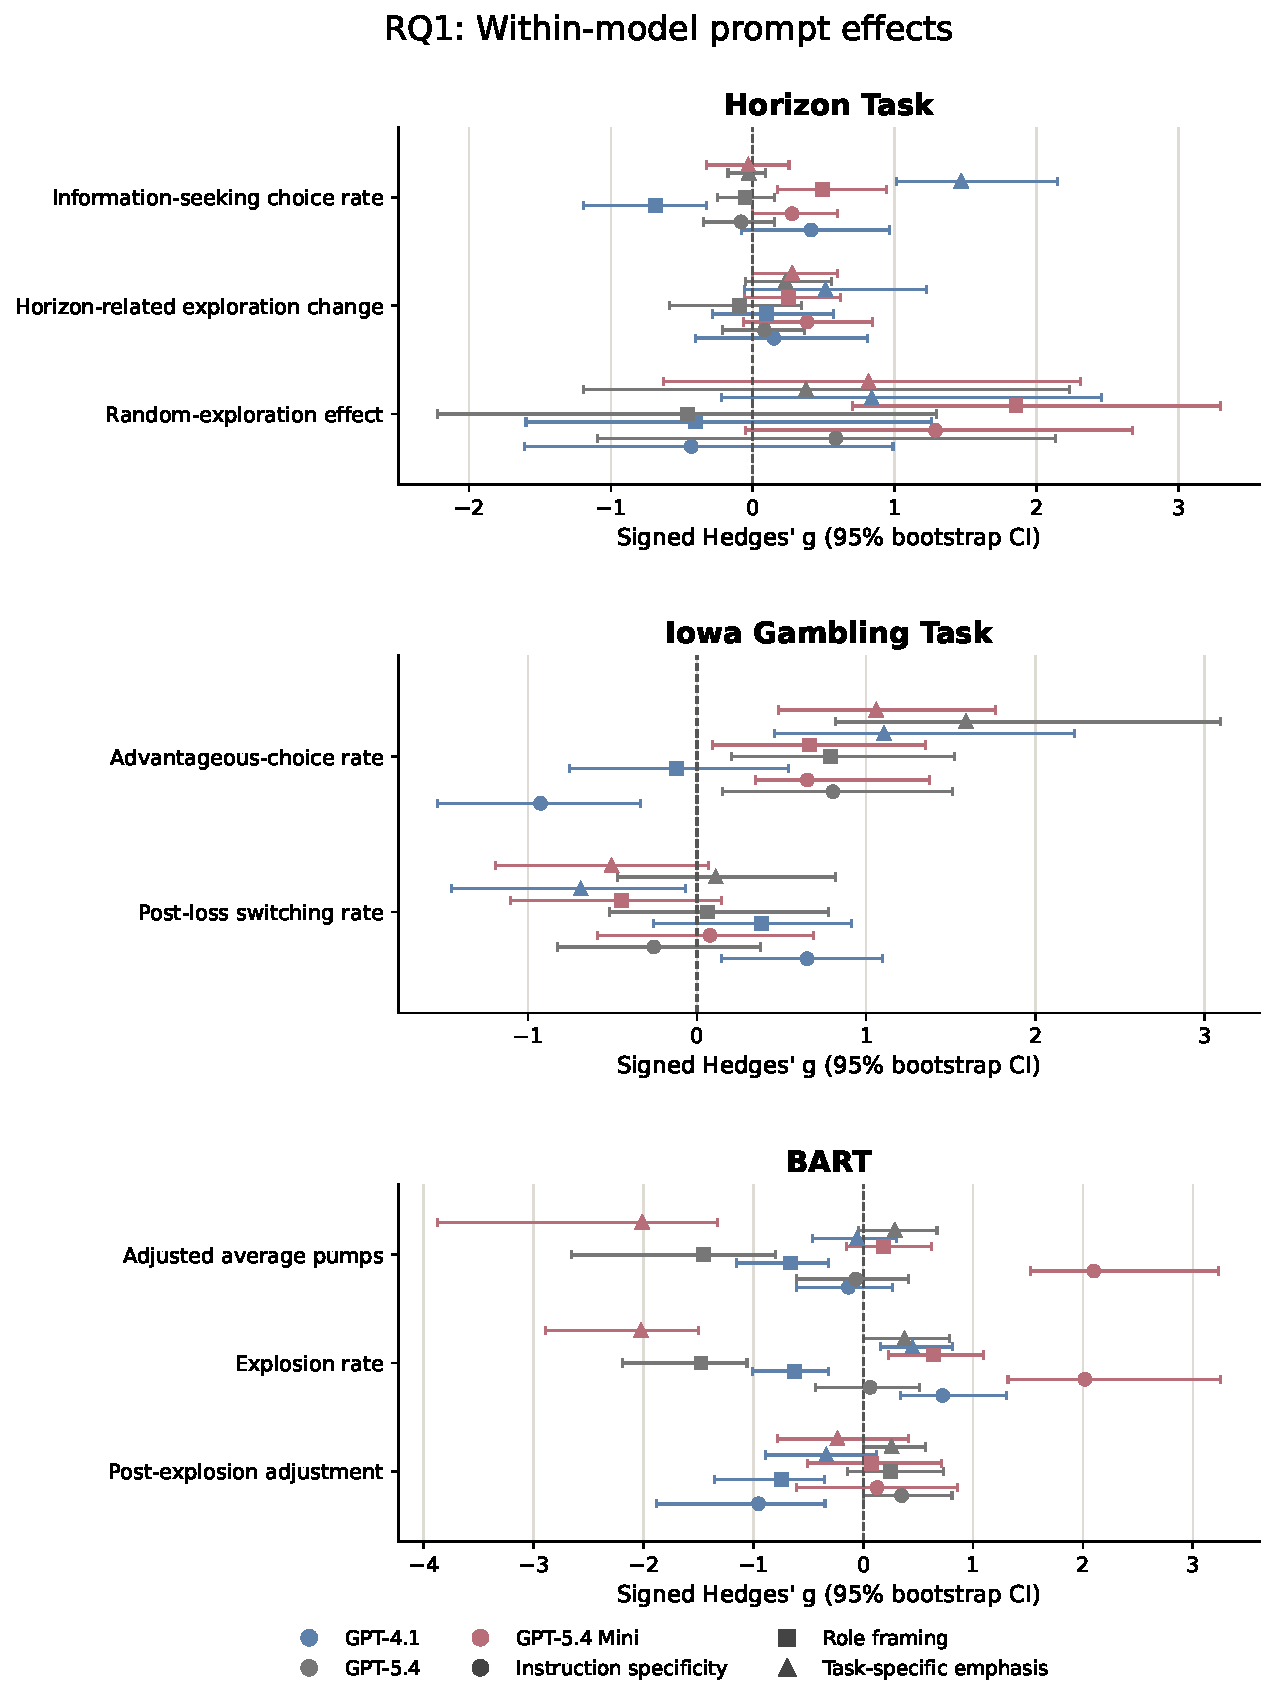
\includegraphics[width=\textheight]{outputs/figures/final_results_v01/figure_rq1_prompt_effects_overview.pdf}
\caption{Task-grouped forest plots of within-model prompt effects relative to Neutral (RQ1). Horizon, IGT, and BART are arranged as three horizontal panels. Points are signed Hedges' $g$ estimates and horizontal lines are percentile-bootstrap 95\% confidence intervals; colour and shape identify model. Raw effects, raw confidence intervals, and PSI are reported in the supplementary tables.}
\label{fig:rq1}
\end{sidewaysfigure}

\begin{sidewaysfigure}[p]
\centering
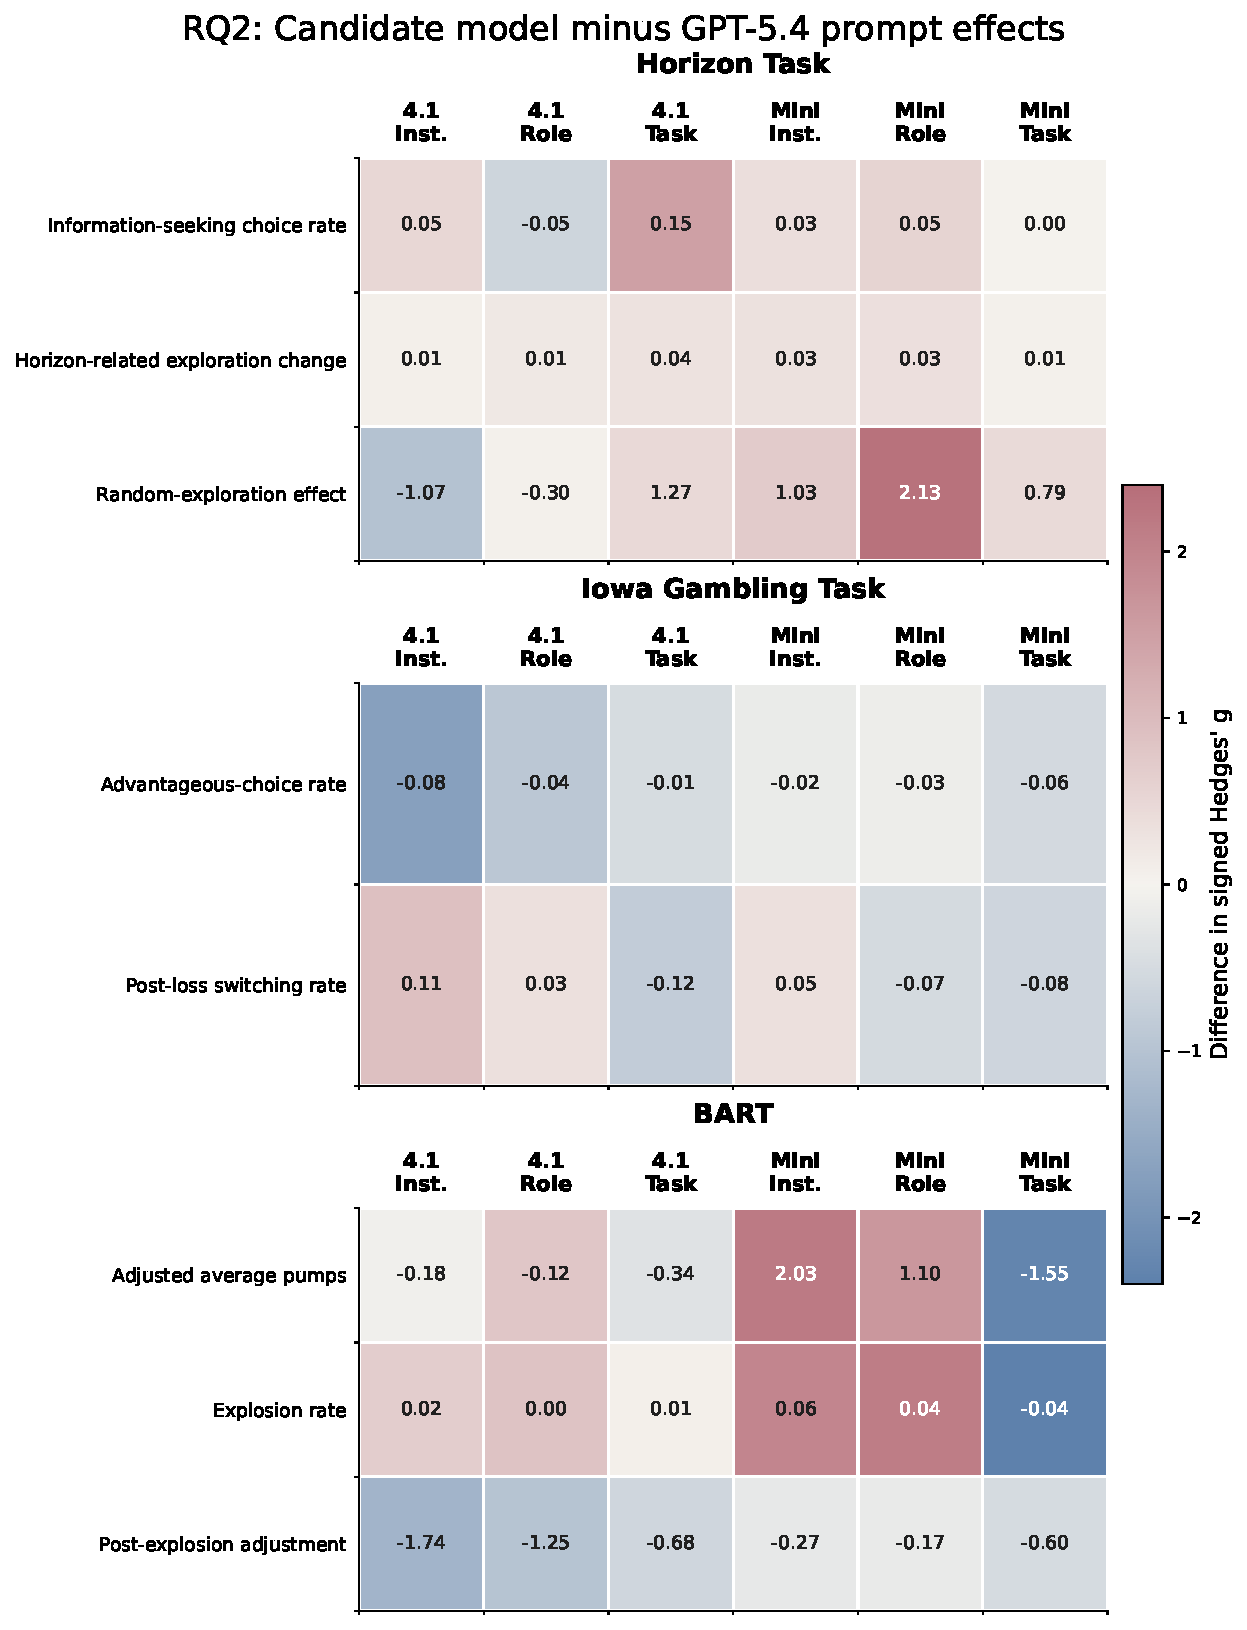
\includegraphics[width=\textheight]{outputs/figures/final_results_v01/figure_rq2_model_interactions_overview.pdf}
\caption{Task-grouped overview of model-by-prompt interaction contrasts (RQ2). Horizon, IGT, and BART are arranged as three horizontal panels. Cell text is the raw interaction $(\bar{Y}_{\mathrm{target},p}-\bar{Y}_{\mathrm{target},N})-(\bar{Y}_{\mathrm{GPT\text{-}5.4},p}-\bar{Y}_{\mathrm{GPT\text{-}5.4},N})$. Colour is the descriptive difference between the two models' signed Hedges' $g$ values. Raw percentile-bootstrap 95\% confidence intervals are reported in the supplementary table; the complete metric-specific forest display is retained in the appendix package.}
\label{fig:rq2}
\end{sidewaysfigure}

\begin{sidewaysfigure}[p]
\centering
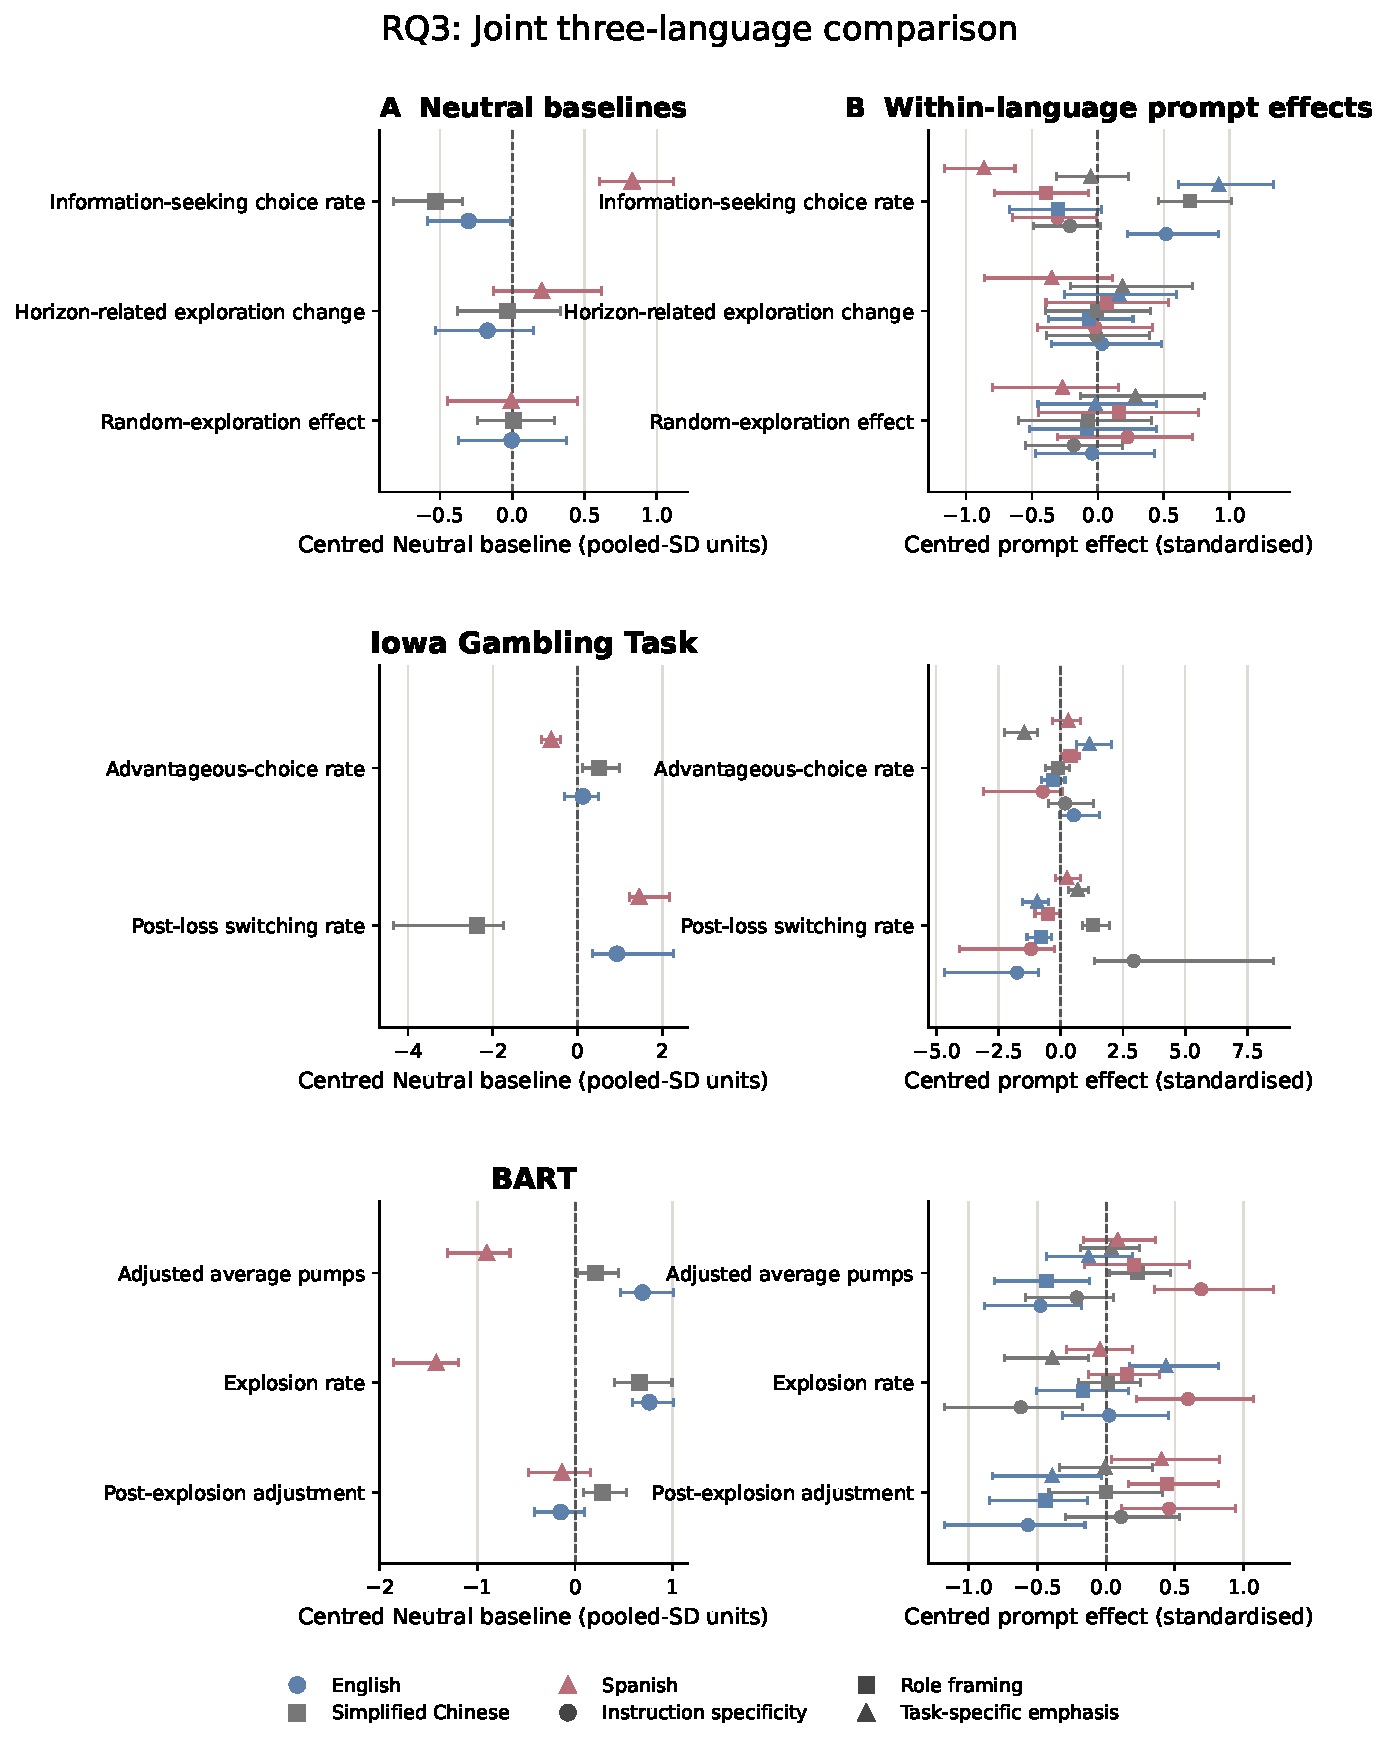
\includegraphics[width=\textheight]{outputs/figures/final_results_v01/figure_rq3_language_overview.pdf}
\caption{Task-grouped forest plots for the joint GPT-4.1 three-language comparison (RQ3). Columns distinguish Horizon, IGT, and BART. The upper row plots each language's Neutral mean deviation from the three-language mean, scaled by the pooled within-language run SD. The lower row plots each language's Hedges' $g$ minus the corresponding three-language mean Hedges' $g$. Both rows include percentile-bootstrap 95\% confidence intervals; the three language-specific deviations sum to zero within each comparison, so no language is designated as a reference. Raw centred estimates and intervals are reported in the supplementary tables.}
\label{fig:rq3}
\end{sidewaysfigure}

\begin{sidewaysfigure}[p]
\centering
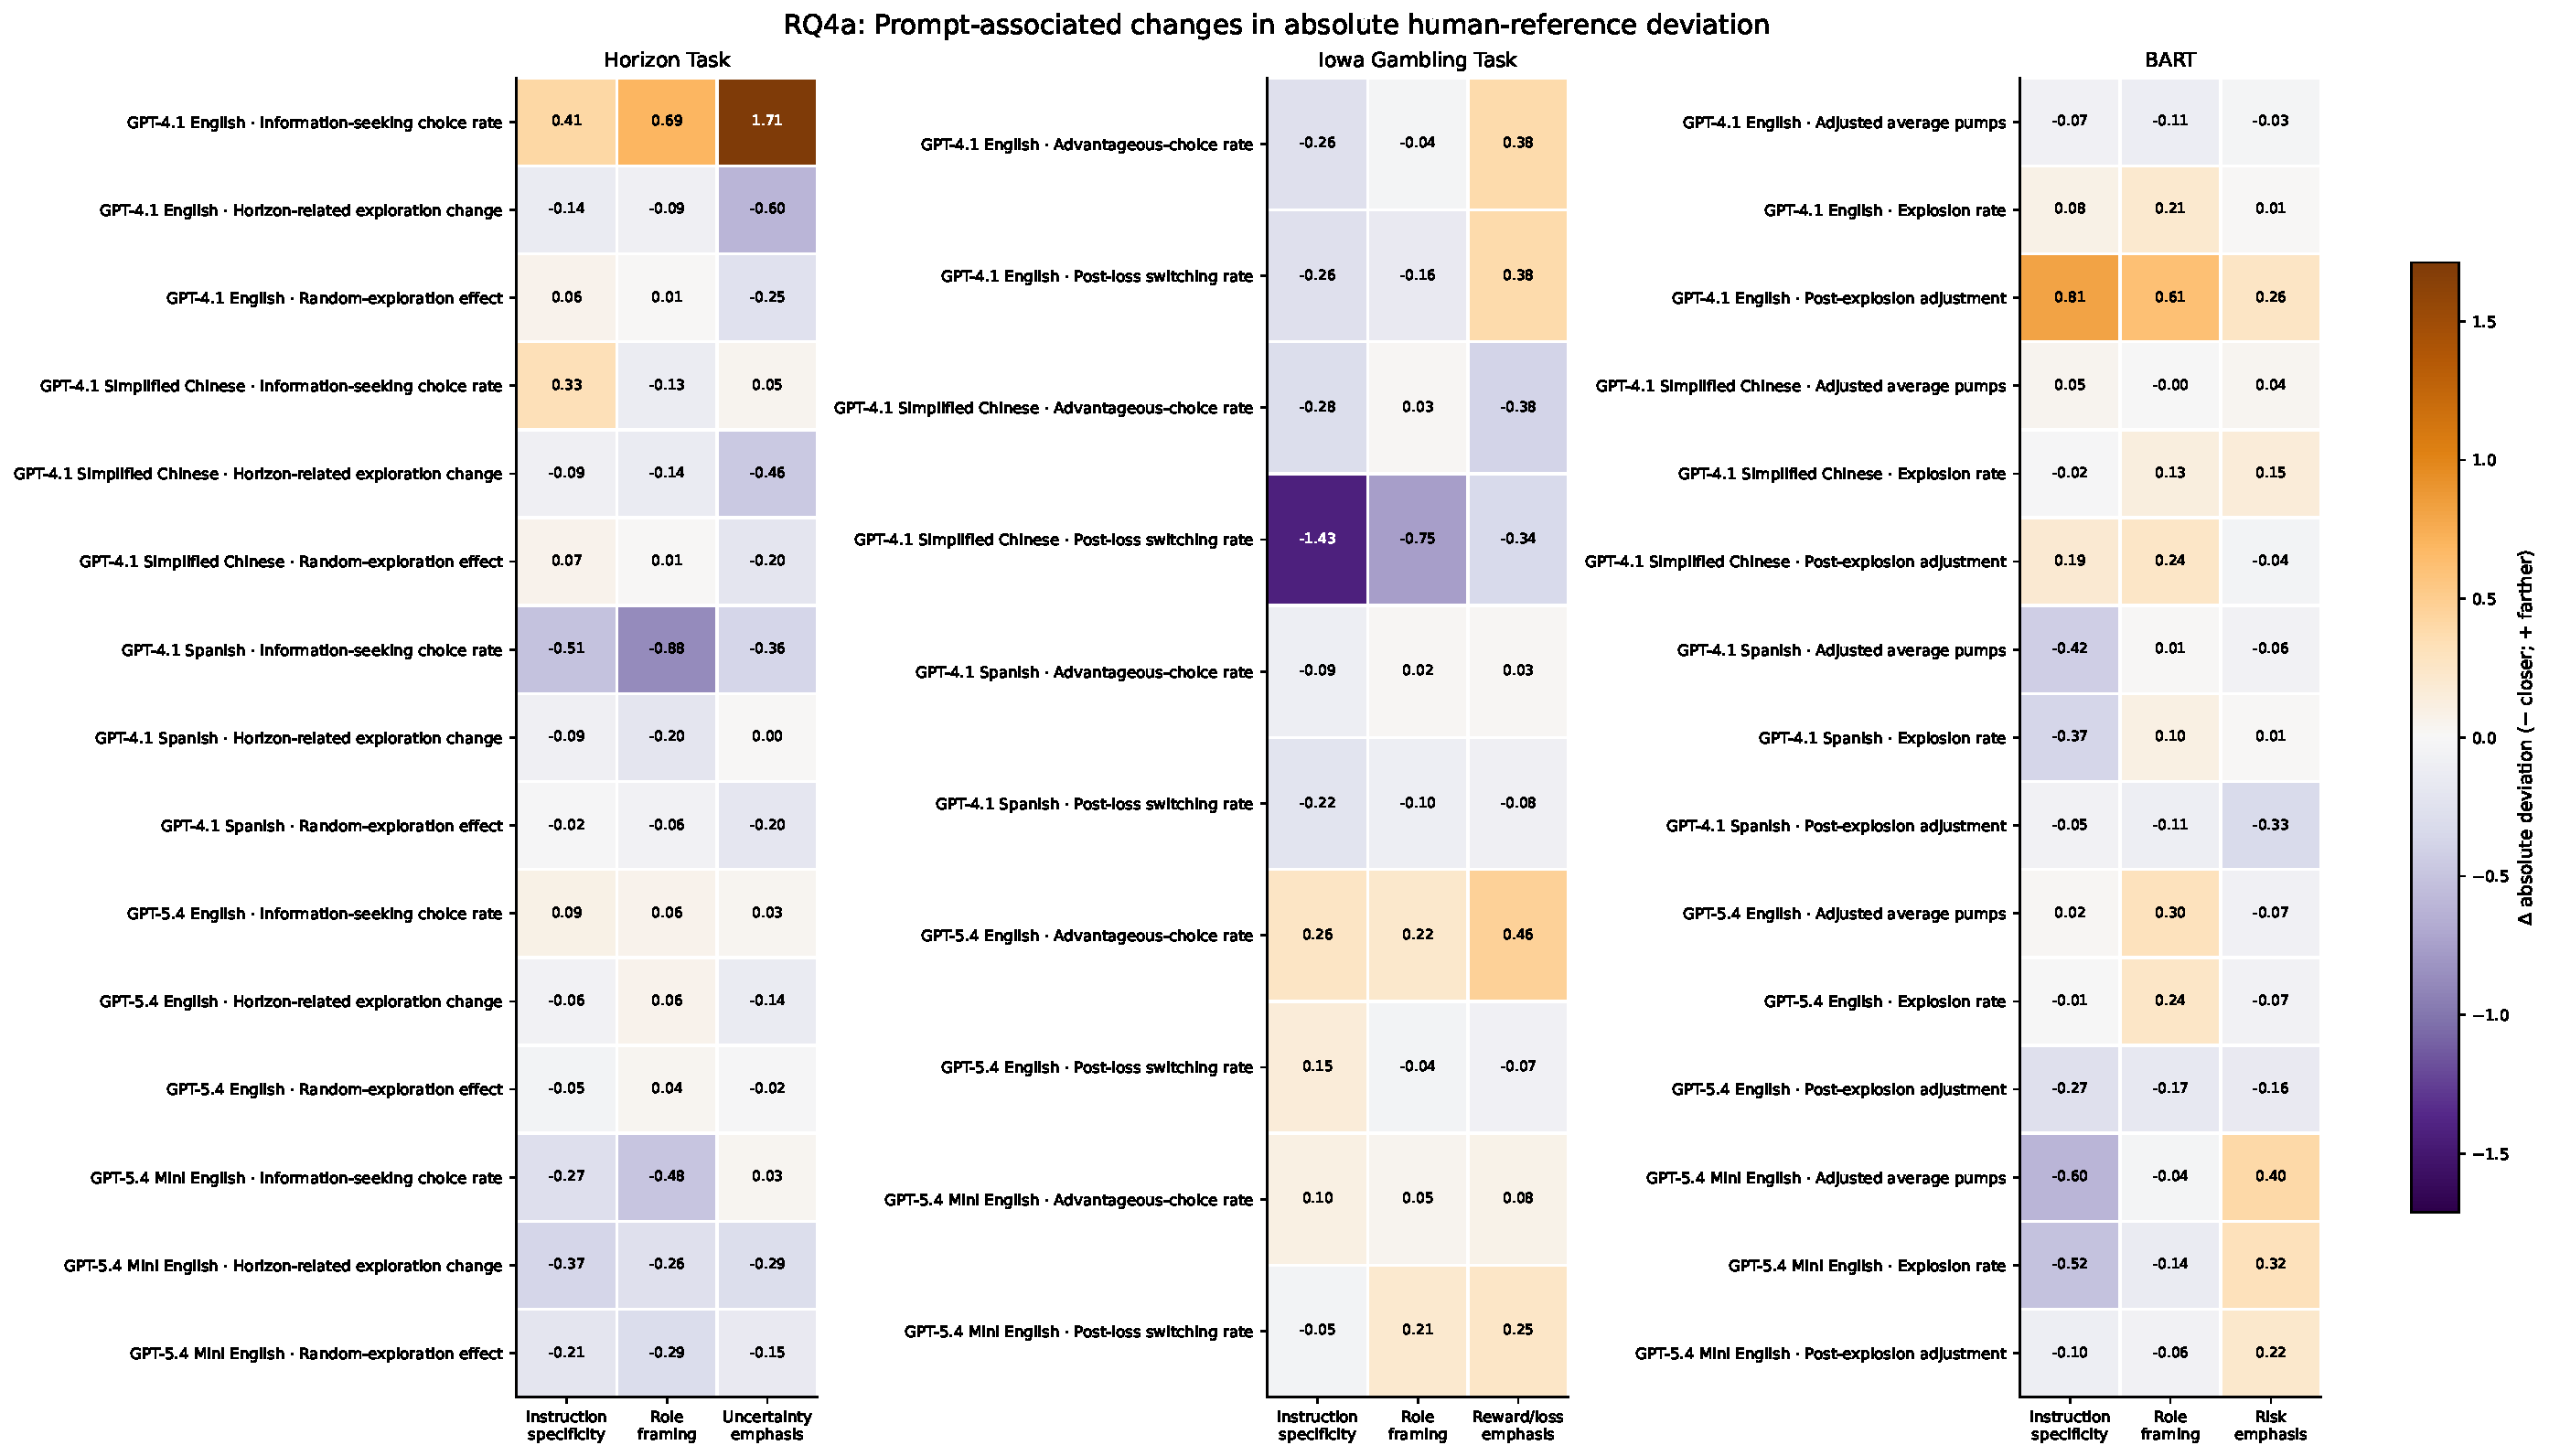
\includegraphics[width=\textheight]{outputs/figures/final_results_v01/figure_rq4_absolute_deviation_heatmap.pdf}
\caption{Prompt-associated changes in absolute human-SD-scaled mean deviation (RQ4a). Cells contain descriptive point-estimated manipulated-minus-Neutral changes: negative values indicate movement closer to the human mean and positive values movement farther away. No inferential intervals were constructed for these human-reference proximity measures.}
\label{fig:rq4a}
\end{sidewaysfigure}

\begin{sidewaysfigure}[p]
\centering
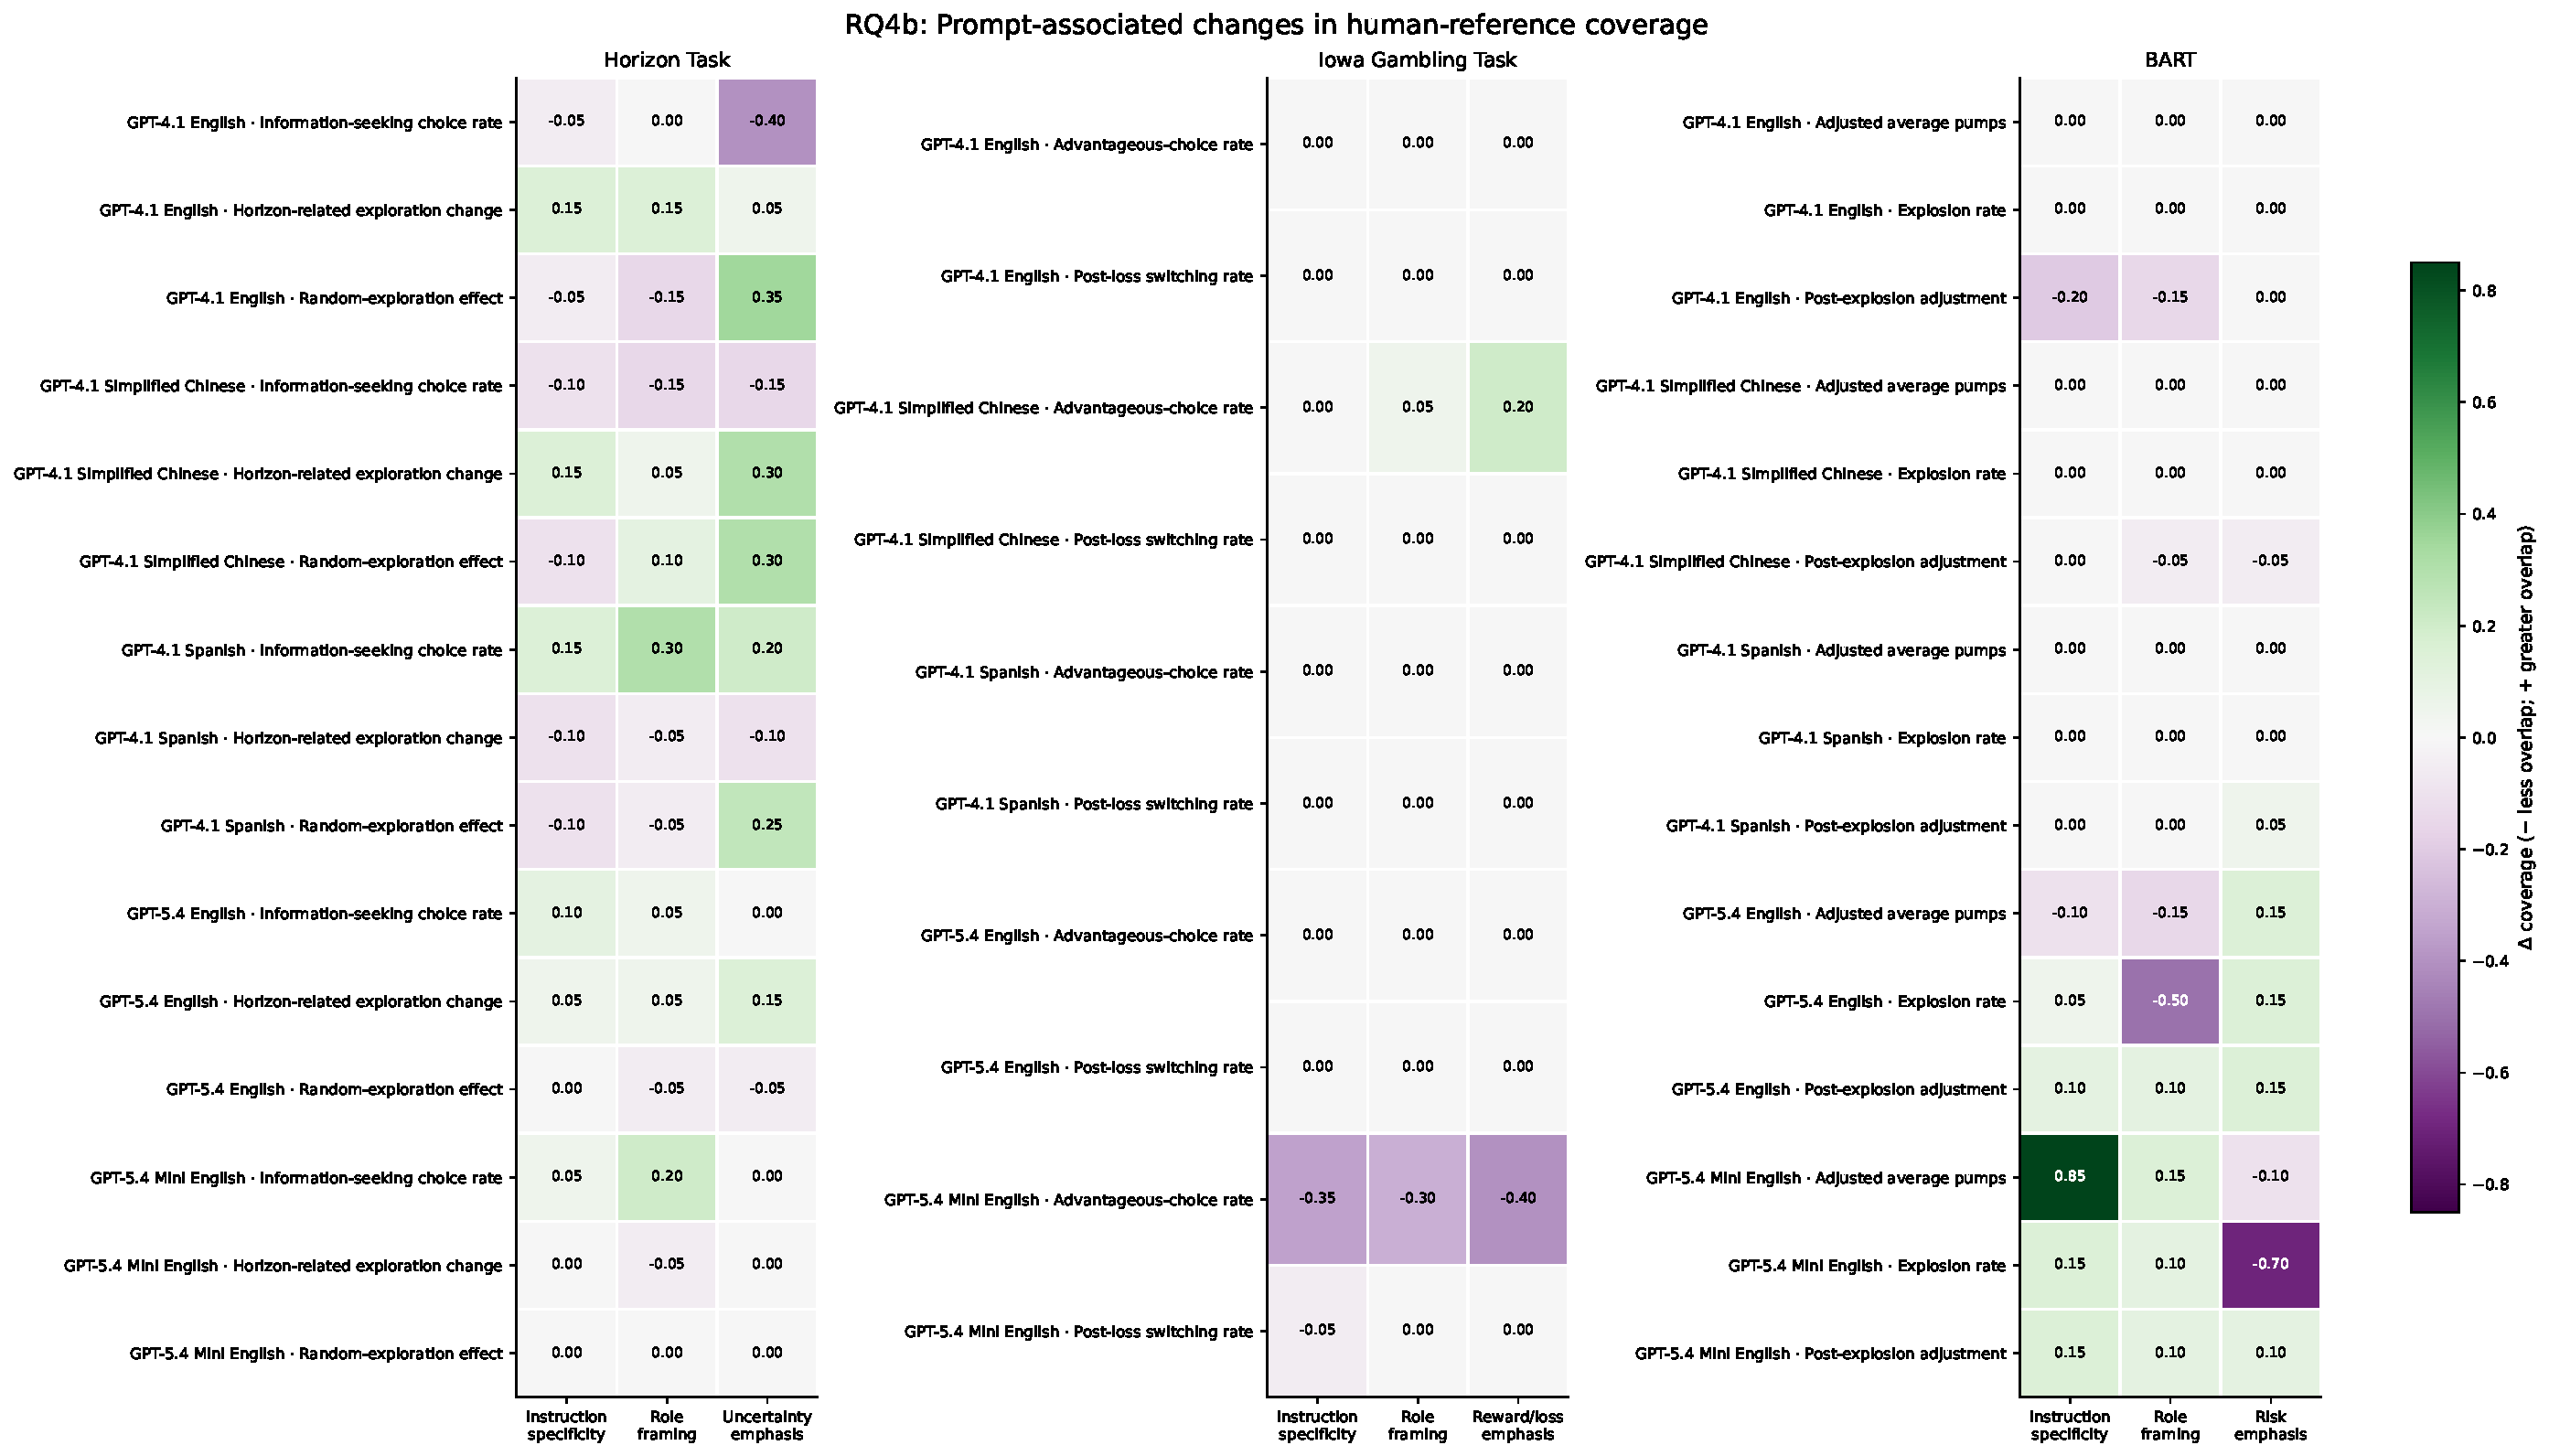
\includegraphics[width=\textheight]{outputs/figures/final_results_v01/figure_rq4_coverage_heatmap.pdf}
\caption{Prompt-associated changes in empirical human-reference coverage (RQ4b). Cells contain descriptive point-estimated manipulated-minus-Neutral changes: positive values indicate greater overlap with the empirical human range and negative values less overlap. Coverage is quantised by the valid-run denominator (in increments of 0.05 when all 20 runs are non-missing). No inferential intervals were constructed for these human-reference proximity measures; neither RQ4 display is an equivalence test or evidence of a shared mechanism.}
\label{fig:rq4b}
\end{sidewaysfigure}


\section{Analysis Sample and Data Quality}

The formal analyses included 1,200 unique, valid, complete task runs; the sample composition and data-quality checks are summarised in Table~\ref{tab:results_quality}. The 240 English GPT-4.1 runs contributed to both the cross-model and cross-language analyses but were counted only once in the total. Each model--language--task--prompt cell contained 20 valid runs. All 480 Simplified Chinese and Spanish runs were ultimately parsed successfully, with no invalid responses. One GPT-5.4 Mini run was parsed successfully after a single prespecified repeat request. Raw-response payloads were not retained for three other unsuccessful attempts, although the audit records preserve the model, task, prompt condition, logical run identifier, failure status, collection time, and mapping to the corresponding replacement run.

All analysis cells passed the prespecified completeness checks. Every formal effect, interaction, and language contrast yielded 2,000 valid bootstrap replicates out of 2,000 requested and met the reporting threshold. No formal cell in this dataset had a pooled standard deviation of zero. All contrasts were prespecified, but no family-wise error-rate or false-discovery-rate correction was applied. Whether an interval includes zero is therefore used only to describe estimation uncertainty, not as a series of independent confirmatory significance tests. Table~\ref{tab:rq_summary} summarises the principal findings and interpretive boundaries for the four research questions.

The random-exploration model converged for the human reference and for every formal LLM cell. The human and LLM analyses used the same model specification, coding, estimation level, and maximum-a-posteriori procedure. All sensitivity fits with shrinkage standard deviations of 0.25, 0.5, and 1.0 also converged. Nevertheless, the magnitude of the estimates varied with the shrinkage setting, so the corresponding standardised effects and human-reference comparisons are treated as model-dependent descriptive results.

\section{RQ1: Within-Model Prompt Sensitivity}

Figure~\ref{fig:rq1} presents forest plots, faceted by task, of signed standardised Hedges' \(g\) values and their 95\% bootstrap confidence intervals. By contrast, the numerical examples below are raw condition-minus-Neutral effects expressed in the original units of each outcome and therefore cannot be read directly from the figure's \(g\) axis. No formulation produced effects of a consistent direction and magnitude across all three models and all outcomes. GPT-4.1's Horizon Task behaviour was particularly responsive to construct emphasis: relative to Neutral, Role framing reduced the information-seeking choice rate by 0.0575 (95\% bootstrap CI [-0.0876, -0.0275]), whereas uncertainty emphasis increased it by 0.1450 ([0.0975, 0.1950]). GPT-5.4's Horizon effects were generally closer to zero, although its IGT advantageous-choice rate increased under all three manipulated conditions.

Model differences were especially apparent in BART. For GPT-5.4, Role framing reduced adjusted pumps by 0.9730 ([-1.2887, -0.6304]). For GPT-5.4 Mini, the Detailed condition increased this outcome by 1.9763 ([1.5780, 2.3926]), whereas risk emphasis reduced it by 1.3114 ([-1.5612, -1.0662]); explosion rate showed corresponding reversals in direction. Advantageous choices and post-loss switching in the IGT did not invariably move together either. The overall answer to RQ1 is therefore that prompt sensitivity was widespread, but its direction and magnitude depended on the model--task--metric combination rather than yielding a uniform ranking of formulations. The PSI serves only as a supplementary summary of this outcome-specific pattern.

\section{RQ2: Cross-Model Variation in Prompt Effects}

Figure~\ref{fig:rq2} summarises direct model-by-prompt interactions with GPT-5.4 as the reference model. They are calculated as \((\text{candidate model: condition}-\text{Neutral})-(\text{GPT-5.4: condition}-\text{Neutral})\); a positive value denotes a more positive prompt effect for the candidate model. The matrix indicates that between-model differences were concentrated in several structured regions rather than taking the form of a common amplification or attenuation of all prompt effects. Differences between GPT-4.1 and GPT-5.4 were most apparent for Horizon information seeking, IGT advantageous choices, and BART post-explosion adjustment. For the latter outcome, the interaction under the BART Detailed condition was -1.7361 pumps ([-2.6121, -0.8463]).

Differences between GPT-5.4 Mini and GPT-5.4 were more concentrated in BART. The adjusted-pumps interaction was 2.0260 ([1.4853, 2.5801]) under the Detailed condition and -1.5486 ([-1.8790, -1.1836]) under risk emphasis, accompanied by a reversal in the direction of explosion-rate effects. For Horizon Role framing, the Random-exploration interaction was 2.1337 ([0.7465, 3.6430]). These contrasts assess whether models responded differently to the same formulation manipulation; they do not assess differences in general capability or baseline behaviour.

\section{RQ3: Cross-Language Variation}

Figure~\ref{fig:rq3} presents the three languages jointly and gives them equal status. Panel A shows pooled-SD-scaled centred baseline deviations, whereas Panel B shows the centred deviation of each language's Hedges' \(g\) from the three-language mean \(g\). The numerical examples below are raw centred deviations in the original units of each outcome and therefore cannot be read directly from the standardised horizontal axes. Panel A locates each language's Neutral mean relative to the common three-language mean. For example, the raw centred baseline deviations in Horizon information-seeking rate were -0.0267 (95\% bootstrap CI [-0.0533, -0.0008]) for English, -0.0467 ([-0.0675, -0.0300]) for Simplified Chinese, and 0.0733 ([0.0500, 0.0958]) for Spanish. The corresponding deviations for IGT post-loss switching were 0.0781, -0.2000, and 0.1219. Within every comparison, the three deviations sum to zero.

Panel B shows the centred deviation of each within-language prompt effect from the mean prompt effect across the three languages for the same task, condition, and outcome. For the effect of Horizon uncertainty emphasis on information seeking, these deviations were 0.0908 ([0.0600, 0.1225]) for English, -0.0067 ([-0.0300, 0.0183]) for Simplified Chinese, and -0.0842 ([-0.1067, -0.0600]) for Spanish. The corresponding deviations for the effect of IGT reward--loss emphasis on advantageous choices were 0.0593, -0.0617, and 0.0023. The Spanish deviation for adjusted pumps under the BART Detailed condition was 0.9073 ([0.4254, 1.4286]). The three-language profiles varied across tasks and outcomes. RQ3 therefore identifies variation in both baseline location and prompt response without assigning reference status to any language. All estimates are restricted to language-associated variation under the present GPT-4.1 snapshot and semantically aligned prompts.

\section{RQ4: Prompt-Associated Changes in Human-Reference Proximity}

Figures~\ref{fig:rq4a}--\ref{fig:rq4b} show changes in absolute human-SD-scaled mean deviation and empirical coverage, respectively. RQ4 reports descriptive point estimates only; no inferential confidence intervals were constructed. Coverage uses the non-missing runs in each cell as its denominator, so the resolution of a cell's coverage is \(1/n_{\mathrm{valid}}\), or 0.05 when all 20 runs are valid. The possible values of \(\Delta C\) depend on the valid denominators in both the Neutral and manipulated cells. Both heat maps contain positive and negative cells, and no formulation consistently improved human-reference proximity across every model, language, and outcome. The labels ``closer'' and ``further away'' refer solely to the direction of the point-estimate change in absolute deviation: negative values indicate greater proximity and positive values greater deviation. This classification does not rely on a bootstrap interval or significance criterion and does not constitute a model ranking.

The larger changes remained strongly conditional. For English GPT-4.1, Horizon uncertainty emphasis increased the absolute deviation in mean information-seeking rate by 1.711 human-SD units and reduced coverage by 0.40. For Simplified Chinese GPT-4.1, the IGT Detailed condition reduced the absolute deviation in post-loss switching by 1.428 human-SD units, while leaving coverage unchanged. For GPT-5.4 Mini, the BART Detailed condition reduced the absolute deviation in adjusted pumps by 0.602 and increased coverage by 0.85. Mean deviation and coverage did not always move together, consistent with their definitions: one describes the location of the cell mean, whereas the other describes the overlap between run-level values and the empirical human range.

\chapter{Discussion}
\label{sec:discussion}

\section{Integrated Findings and Methodological Contribution}

The principal finding is not that any one prompt formulation universally strengthens or weakens a class of behaviour. Rather, behavioural conclusions are conditional on the complete measurement specification. RQ1 showed that the direction and magnitude of a formulation's effect varied across models, tasks, and outcomes. RQ2 further showed that baseline differences or broad claims about model capability cannot substitute for this analysis, because models differed in the structure of their responses to the same manipulation. RQ3 characterised both centred baseline locations and centred within-language prompt effects across the three languages. RQ4 showed that prompts could also shift human-reference proximity, and that mean deviation and empirical coverage capture distinct properties. Results obtained with a single prompt, snapshot, or language therefore cannot automatically be treated as stable attributes of the model's task behaviour. Consequently, these systems are not reliable cognitive models in the strong sense of exhibiting prompt-invariant behavioural properties; their reliability is conditional and must be established for a specified model, prompt, task, language, outcome, and collection context.

The methodological contribution should be understood alongside this finding. The study treats the complete task run as the unit of replication and combines controlled prompt variants, direct model interaction contrasts, and symmetric three-language centred comparisons within a single framework. Matched task-environment seeds and their block bootstrap apply only to the Horizon Task and BART; IGT runs are resampled independently within the relevant cells; and hierarchical refitting is confined to the Horizon Random-exploration estimator. The aim is not to produce a general reliability score spanning tasks, but to identify the model--language--task--condition--metric combinations under which a conclusion remains stable or changes. Raw task outcomes consequently remain the principal units of interpretation, with the PSI and standardised graphics serving only to aid navigation across outcomes.

\section{Conditionality of LLM Behavioural Measurement}

Prompt sensitivity should not be dismissed as irrelevant noise. Instruction specificity, Role framing, and Task-specific construct emphasis alter the informational cues supplied by the measurement procedure. A response pattern can be behaviourally interpretable while still demonstrating that the conclusion depends on its formulation. Template and format sensitivity have already been documented in static benchmarks~\cite{Sclar2024PromptFormatting,Mizrahi2024MultiPrompt,Hua2025FlawArtifact}. The present results extend that evidence by showing that such dependence can accumulate in run-level behavioural summaries generated through sequential choices, and that outcomes can diverge within the same condition. Robustness does not require every prompt to produce identical output; it requires researchers to establish which conclusions persist across prespecified formulations with matched informational boundaries.

The model and language results broaden this boundary. Differences between snapshots were concentrated in particular behavioural components and did not yield a uniform ranking of models by robustness. Moreover, changes in proprietary services restrict attribution to the recorded snapshots and collection periods~\cite{Chen2024ChatGPTBehavior,Palmer2024ProprietaryModels}. Cross-language variation likewise involved both baseline location and response to the manipulation, and cannot be characterised by comparing manipulated-condition means alone. Translation length, word order, keyword salience, pragmatic convention, and collection time cannot be fully separated from an abstract language system. The results are accordingly interpreted as language-associated variation rather than as pure language effects.

Cross-task comparison serves to delimit interpretation, not to rank the tasks. Horizon information seeking, horizon-related change, and model-derived Random exploration are distinct operationalisations. IGT advantageous choices and post-loss switching describe different responses to feedback, just as BART pumps, explosions, and post-explosion adjustment do not share a single normative direction. Their separation in the figures suggests that formulations affect particular components of behavioural organisation rather than general ``performance''. A larger effect, a greater number of pumps, or a higher information-seeking rate therefore cannot be labelled better, more rational, or more similar to human cognition without reference to the outcome definition.

\section{Human Reference and Interpretive Boundaries}

Human-reference comparisons provide an external descriptive coordinate, not a test of mechanism. Mean deviation locates the cell mean relative to the human mean, whereas coverage measures the overlap between run-level values and the empirical human range. Their failure to move together is not contradictory because they describe different objects. Research on behavioural similarity between humans and models has likewise emphasised the need to distinguish similarity of outputs from equivalence of mechanisms~\cite{Lampinen2024ContentEffects,Lin2025SixFallacies}. A smaller human-SD-scaled deviation is therefore not interpreted here as evidence of a shared cognitive process, nor is greater coverage taken to imply that the LLM runs form a human participant distribution.

The same restriction applies to the unit of analysis. Run-level replication estimates behavioural variability across repeated generations under a fixed model and deployment setting. The runs share model parameters and a deployment environment; their differences arise from task states, context, and generation stochasticity. Treating runs as analytical replicates is therefore not equivalent to sampling independent members of a synthetic population, and runs should not be regarded as independent synthetic participants. Operational alignment between human-participant and LLM-run summaries permits descriptive comparison, but does not resolve population representativeness, individual differences, or mechanism identification~\cite{Dillion2023ReplaceParticipants,Bisbee2024SyntheticSurveyData}. RQ4 consequently asks whether a prompt changes a result's position relative to a human reference, not whether a model is ``human-like''.

\section{Limitations, Reproducibility Implications, and Future Work}

The study's inferences are first constrained by its design. Twenty runs per cell permit estimation of the prespecified contrasts in the present design, but precision remains limited and the sample cannot adequately characterise rare strategies, distributional tails, or high-dimensional interactions. Bootstrap resampling cannot compensate for a small cell size or establish adequate statistical power. Internal deployment details and subsequent changes to proprietary API snapshots are not fully observable to researchers, and no sampling seed is available to reproduce token-level generation. The semantic prompt manipulations also cannot be fully separated from length, repetition, position, and keyword salience. Multilingual review established task-relevant informational equivalence, not complete translational or cultural equivalence; the later collection of the Chinese and Spanish samples may also introduce temporal drift.

The human-reference analyses are additionally limited by imperfect alignment between task implementations and reference estimation. The human datasets and LLM runs differ in task length, familiarisation, and information presentation. RQ4 treats the human mean, standard deviation, and empirical quantiles as fixed descriptive references and does not propagate their sampling uncertainty. Its conclusions are therefore conditional on the selected datasets, sample moments, and empirical quantiles; they cannot be generalised directly to a wider human population or to other reasonable reference datasets. Although Random exploration used an aligned model specification, its magnitude was sensitive to the shrinkage setting. Finally, because the study did not apply multiplicity-adjusted hypothesis tests across the many related contrasts, no isolated interval or strongly shaded cell should be regarded as independent confirmatory evidence.

These limitations imply several direct requirements for replication. Prompts should be versioned as experimental materials, and studies should report multiple theoretically meaningful formulations with matched informational boundaries. Cross-model questions require direct interaction estimates, whereas cross-language questions should locate all languages jointly in a common coordinate system rather than comparing separate intervals. Complete runs, parser repairs, failed attempts, resolved model identifiers, collection dates, and bootstrap diagnostics should remain available for audit. Future work should examine independent snapshots and larger cell sizes, prespecify narrower comparison families, and use orthogonal manipulations to separate semantic content from prompt length and keyword salience. Such studies would establish whether the conditional patterns observed here persist across service updates and task implementations.

Taken together, the evidence does not support a prompt ranking that remains constant across conditions. It supports a narrower, auditable conclusion: LLM results in decision-making tasks show systematic but task-specific sensitivity to the measurement specification. Reliable use of such evidence requires joint reporting of the formulation, model snapshot, language, behavioural outcome, and uncertainty, while retaining human-reference proximity as a conditional descriptive comparison.

\chapter{Conclusion and Future Work}
\label{sec:conclusion}

How reliable, then, are LLMs as cognitive models? Under the behavioural definition adopted in this dissertation, the answer is conditional. The tested systems cannot be regarded as reliably prompt-invariant models of cognition: observed effects varied across model snapshots, tasks, outcomes, and language implementations, and the same prompt manipulation could produce changes in opposite directions across models or outcomes. They can nevertheless serve as useful computational models of cognitive-task behaviour when claims are restricted to an explicit measurement specification and their robustness is evaluated across prespecified formulations. Prompt sensitivity was structured and conditional, rather than a general effect captured by a single ranking of formulations; claims about exploration, response to feedback, or risk taking should therefore not be generalised directly from one prompt, model snapshot, or language implementation.

The study's principal contribution is an auditable evaluation framework for locating this conditionality. It treats a complete task run as the unit of repeated generation, compares prespecified prompt variants with matched informational boundaries, directly estimates cross-model interaction contrasts and three-language centred deviations, and distinguishes task-specific behaviour, prompt sensitivity, and human-reference proximity. The human-reference analyses further show that the proximity of a cell mean to the human mean and the overlap of run-level values with an empirical human range can change separately across prompts. Both are descriptive references: neither demonstrates a shared cognitive mechanism nor establishes distributional equivalence between LLM runs and the human participant population.

Future work should prioritise replication at different collection times and across additional model snapshots, together with larger numbers of runs per cell to improve the precision of estimates for variable outcomes, rare strategies, and interaction effects. Orthogonal designs could then separate the contributions of semantic emphasis, prompt length, information position, and keyword salience. Multilingual research would benefit from independent translation validation and more closely synchronised data collection to reduce confounding between translation implementation and temporal drift. Human-reference analyses should propagate uncertainty in the human reference statistics and more closely align task length, information presentation, and measurement precision. By releasing prompts, model and collection-version information, the full analysis workflow, parser repairs, and failed-attempt records, future studies can more reliably distinguish behavioural regularities that persist across measurement implementations from findings produced by a particular experimental configuration.

\bibliographystyle{plain}
\bibliography{final_references}

\end{document}
